% TLP2esam.tex / sample pages for TLP
% v2.11, released 6-nov-2002

\documentclass{tlp}
\usepackage{ifthen}
\usepackage{url}
% Remove hyperref for final version!!
% \usepackage[pdftex,colorlinks=false,urlcolor=blue]{hyperref}
\usepackage{swipl}
\usepackage{amssymb}
\usepackage{upgreek}
\usepackage{color}
\usepackage{textcomp}

\usepackage{listings}


\lstset{
  basicstyle=\ttfamily,
  columns=fixed,
  fontadjust=true,
  basewidth=0.5em,
  xleftmargin=0.5em,
  captionpos=b
}

\newcommand{\authornote}[3]{{\color{#2} {\sc #1}: #3}}
\newcommand\jan[1]{\authornote{jan}{red}{#1}}
\newcommand\TODO[1]{\authornote{TODO}{red}{#1}}

\newcommand\cplint{\texttt{cplint}}
\newcommand\cplintonswish{\cplint{} on SWISH}

\usepackage[pdftex]{graphicx}
\DeclareGraphicsExtensions{.pdf,.jpg,.png}
\graphicspath{{figs/}{./}}
\newcommand{\tag}[1]{\texttt{#1}}
\newcommand{\fnurl}[1]{\footnote{\url{#1}}}
\sloppy

\begin{document}
\bibliographystyle{acmtrans}

\title{Web Prolog and the programmable Prolog Web}


\author[T. Lager]
{TORBJ\"ORN LAGER \\
University of Gothenburg\\
\email{lager@ling.gu.se}
}

\pagerange{\pageref{firstpage}--\pageref{lastpage}}
\volume{\textbf{?} (?):}
%\jdate{August 2007}
\setcounter{page}{1}
%\pubyear{2007}

\maketitle
\begin{abstract}
We describe a programming language called \textit{Web Prolog}. We think of it as a \textit{web programming language}, or, more specifically, as a web \emph{logic} programming language. The language is based on Prolog, with a good pinch of Erlang added. We stay close to traditional Prolog, so close that the vast majority of programs in Prolog textbooks will run without modification. Towards Erlang we are less faithful, picking only features we regard as useful in a web programming language, e.g. features that support concurrency, distribution and intra-process communication. In particular, we borrow features that make Erlang into an \textit{actor programming language}, and on top of these we define the concept of a \textit{pengine} -- a programming abstraction in the form of a special kind of actor which closely mirrors the behaviour of a Prolog top-level. On top of the pengine abstraction we develop a notion of \textit{non-deterministic RPC} and the concept of \textit{the Prolog Web}.
\end{abstract}


\begin{keywords}
Prolog, Erlang, SCXML, web programming
\end{keywords}

%\newpage
%\subsection*{Temporary!}
%\tableofcontents
%\newpage

\section{Introduction}\label{s1}

\noindent Readers with a background in computational logic are more than likely familiar with Prolog, and with programs written in the following style:

\begin{lstlisting}
human(X) :- rational(X), animal(X).

rational(socrates).     animal(socrates).
rational(plato).        animal(plato).
rational(aristotle).    animal(aristotle).
\end{lstlisting}

\noindent In first-order logic (FOL) the first clause would translate into $\forall x [rational(x) \land animal(x) \rightarrow human(x)]$.

In a suitable Prolog shell, queries such as the following can be asked:

\begin{lstlisting}
?- human(Who).
Who = socrates ;
Who = plato ;
Who = aristotle.
?-
\end{lstlisting}

\noindent In first-order predicate logic this query is equivalent to $\exists x [human(x)]$.

This is \textit{pure} Prolog.

In the years since researchers involved in computational logic disappeared from the field of logic programming and went into the new area of Semantic Web, Prolog has evolved considerably. From a semantic web perspective, \textit{tabling} \cite{??} is perhaps the most useful feature, but there are others, such as constraint logic programming. Prolog is also showing great promise as a web programming language, witness applications such as SWISH \cite{DBLP:journals/corr/abs-1808-08042}. 

As a logic programming language, Prolog represents a programming paradigm which at its core is unique and very different from imperative or functional programming languages. Features such as built-in backtracking search, unification and a built-in clause database form the basis for logic-based knowledge representation and reasoning, and support for meta-programming, user-defined operators, a term-expansion mechanism and grammars is also provided. These are the features that underlie Prolog's reputation as a symbolic AI programming language. 

%-- an attempt to ``plug out'' the sequential part from Erlang and ``plug in'' sequential Prolog instead

%\begin{lstlisting}
%ancestor_of(X,Y) :- parent_of(X,Y).
%ancestor_of(X,Z) :- parent_of(X,Y), ancestor_of(Y,Z).
%
%parent_of(X,Y) :- mother_of(X,Y).
%parent_of(X,Y) :- father_of(X,Y).
%
%mother_of(trude, sally).
%
%father_of(tom,sally).
%father_of(tom,erica).
%father_of(mike,tom).
%\end{lstlisting}

The structure of the paper is as follows. The rest of this section justifies the introduction of yet another dialect of Prolog. Section~\ref{sec:browser} presents an IDE for Web Prolog, introduces the notion of a \textit{node}, and describes the interaction between the IDE and a node over a WebSocket sub-protocol. Section~\ref{sec:language} introduces the language of Web Prolog as such and compares it with Erlang. Section~\ref{sec:beyond-erlang} looks closer at the combination of the actor model and the logic programming model, placing a particular focus on non-determinism and backtracking. The notion of a pengine is described in detail, and a notion of non-deterministic RPC is developed. Section~\ref{sec:previous} describes some earlier work, Section~\ref{sec:discussion} provides a discussion, and Section~\ref{sec:summary} summarises and suggests avenues for further work.


\subsection{Web Prolog is a Hybrid Programming Language}\label{sec:hybrid}

%\begin{quote}
%\noindent Imagine a dialect of Prolog with actors and mailboxes and send and receive -- the means necessary for powerful concurrent and distributed programming. Alternatively, think of it as a dialect of Erlang with logic variables, backtracking search and a  built-in database of facts and rules -- the means for logic programming, knowledge representation and reasoning. Also, think of it as a web logic programming language. This is what Web Prolog is all about.
%\flushright\textit{Web Prolog -- the elevator pitch}
%\end{quote}
%
%\noindent Prolog is a logic programming language. Based on formal logic, a subject dating all the way back to the antiquity and tried and tested by generations of logicians and philosophers, logic programming forms a paradigm of it own. Even in its pure form, as a set of Horn clauses, Prolog is Turing complete but a number of extra-logical constructs has been added to ensure its usefulness as a general purpose programming language.  

\noindent Web Prolog is not only a logic programming language but also an \textit{actor programming language} as it extends Prolog with primitives for spawning processes and sending and receiving messages in the style of Erlang, i.e. constructs that made Erlang such a great language for programming message-passing concurrency and distribution. Provided we can accept using a syntax which is relational rather than functional it turns out that the surface syntax of Prolog can easily be adapted to express them. Since Prolog and Erlang also share many other properties such as dynamic typing, the use of immutable variables, and a reliance on pattern matching and recursion, creating a hybrid between them seems reasonable. (Indeed, it allows us to regard Web Prolog either as a new dialect of Prolog, or as a new dialect of Erlang.)

\subsection{Web Prolog is a Web Programming Language}\label{sec:hybrid}

\noindent There are more than a dozen Prolog systems around, and we do not intend to compete with them, or with Erlang for that matter. Although the proposed hybrid between Prolog and Erlang would likely work as a general-purpose language, this is not what we aim for. Instead, as suggested by the first part of its name and in an effort to find new uses for Prolog, we think of Web Prolog as a special-purpose programming language -- as an embedded, sandboxed scripting language for programming the Web with logic and for implementing web-based communication protocols in the style of Erlang.

%Some twenty-five years in the making, the World Wide Web is a formidable success and the biggest distributed programming system ever constructed, and has, over the years, become a key delivery platform for a variety of sophisticated interactive applications in just about any conceivable domain. By rebranding Prolog as a web programming language we intend to make an attempt to ensure Prolog can be used to build a web endowed with logic and reasoning capabilities. 

Web Prolog is an embedded language, designed to be implemented in a host language running in a host environment. We have embedded our Web Prolog proof-of-concept implementation in SWI-Prolog \cite{wielemaker:2011:tplp} but we are convinced it can also be embedded in other Prolog systems, in systems supporting non-Prolog programming languages or knowledge representation languages, and in web browsers through transpilation into JavaScript or compilation into WebAssembly.

Web Prolog is furthermore a sandboxed language, open to the execution of untested or untrusted source code, possibly from unverified or untrusted clients without risking harm to the host machine or operating system. Therefore, Web Prolog does not include predicates for file I/O, socket programming or persistent storage, but must rely on the host environment in which it is embedded for such features.

\section{Webizing Prolog -- an exercise in
retrofitting}\label{sec:webizing-prolog}

\begin{quotation}
\noindent The essential process in webizing is to take a system which is
designed as a closed world, and then ask what happens when it is
considered as part of an open world. Practically, this effect on a
computer language is to replace the names/tokens/identifiers for URIs.
Thus, where before reference could only be made to something in the
same document/program/module one can with equal ease make reference to
something in a different one somewhere in that abstract space which is
the Web.
\vspace{0cm}
\flushright  \textit{Tim Berners-Lee, 1998}
\vspace{0.2cm}
\end{quotation}

\noindent Here is what might be involved in webizing Prolog in order to obtain the Web Prolog programming language and an architecture for the Prolog Web:

\begin{itemize}

\item As suggested in the above quote from Berners-Lee, webizing a system involves the introduction of URIs as names in a system to scale it to the Web. %As we shall see in the case of Web Prolog and the Prolog Web, it involves URIs pointing to nodes, URIs pointing to actors running on nodes, URIs pointing to answers to queries, and URIs pointing to Web Prolog source code. Such URIs can appear in the arguments of predicates, or as values of options passed in predicates.

\item To be successfully webized, a language and an architecture must exploit the existing web infrastructure. %In the case of Web Prolog and the Prolog Web, this suggest employing protocols such as HTTP and WebSockets, as well as formats such as JSON. In an open network such as the Web, security is of utmost importance, and as we shall see, the existing web infrastructure can provide the Prolog Web with various forms of security. Web browsers should be capable of running Web Prolog

\item In an open network such as the Web, security is of utmost importance.

\item An infrastructure must be scalable to web size.

\item It must fit the web application development paradigm.

\item To be properly webized, a language and an architecture which tries to extend the Web must be standardised. %In order to achieve interoperability Web Prolog demands standardisation on more than one level -- from the pragmatics of interaction all the way down to the syntactic details of the language. 

\item Finally, a system must also fit the web \textit{culture} -- openness and
extensibility and support for communities of interest and practise. %In the case of Web Prolog, it is natural to first and foremost try to establish Web Prolog as a language supporting the Prolog and Logic Programming communities. 

\end{itemize}

\noindent Among Prolog systems, SWI-Prolog in particular has all the right tools for building server-side support for web applications, in the form of mature libraries for protocols such as HTTP and WebSocket, and excellent support for formats such as HTML, XML and JSON. Therefore, it might be argued that since Prolog can and has been used for building server-side support for web applications, it should already be counted as a web programming language. But since this is true also for Python, or Ruby, or Java, or just about any other general-purpose programming language in existence, it would make the notion of a web programming language more or less empty. We could of course argue that SWI-Prolog is much better at providing what is needed, but we shall go further than that. We believe Prolog should claim an even more prominent position in this space. Prolog should be used not only for building server-side support for web applications, but should be considered as \textit{part} of the Web, in much the same way as HTML, CSS, JavaScript, RDF and OWL are parts of the Web. In other words, we want it to be seen as \textit{a web technology in its own right}.

Prolog is a rather old programming language and easily predates the appearance of the Web. This has consequences for how we can go about webizing Prolog. While web logic languages such as RDF and OWL were \textit{designed} for the (Semantic) Web, \textit{retrofitting} might be a more apt description of what we need to do with Prolog.

Webizing has often implied XMLizing. OWL, for example, is a webized ontology language for which an XML-based syntax has been invented. XMLizing Prolog does not make sense (just as it does not make sense for JavaScript). Instead of bringing logic and (aspects of) logic programming to the Web, which is what the semantic web community has done, we argue that it makes sense to bring (nearly) the \textit{whole} of Prolog there. Since XMLizing the whole of Prolog would be a daunting task, and as the result would likely be sub-optimal, we much prefer to stick to the Prolog syntax.


\section{The Prolog Web in a nutshell}\label{sec:prolog-web-in-a-nutshell}

\noindent The Web started out as a distributed hypertext system, but already in its current form, thanks to inventions such as web services and APIs, the Web has also become a simple and flexible environment for distributed programming. At one point in the history of its evolution, the Hypertext Web morphed into a \textit{Programmable Web}. With the help of state-of-the-art web technologies, the Prolog Web tries to take this a step further. The programmable Prolog Web supports two different models for distributed programming, one based on actors and stateful, asynchronous communication over websockets, and one based on the stateless, synchronous communication provided by HTTP. We argue that with the help of these technologies, the Prolog Web can be made \textit{programmable} in an unusually strong sense of this word.

The traditional Web is distributed, decentralised and open. These are traits we want the Prolog Web to also possess. Whereas distribution is nicely conceptualised in the actor model, and nicely handled by an actor programming language such as Erlang, decentralisation and openness require features we must rely on the Web as such to contribute. Erlang and most other platforms for distributed programming are not open in the sense that we require. They usually rely on TCP for transport and are, for reasons of security, assumed to be operating in a closed, trusted environment where we directly control the machines we are operating. In other words, when Erlang runs on a \textit{cluster}, it is a cluster that is \textit{closed} and \textit{static}. We can think of the Prolog Web as a cluster as well, but one that is \textit{open} and \textit{dynamic}. (Note that it is not dynamic in the sense that new node instances are created dynamically, but only in the sense that new \textit{connections} between nodes are dynamically created as needed.)

Naturally, creating a Prolog Web entails adapting Prolog to the current Web rather than the other way around. This is what is meant by webizing, and not only does it involve designing a special-purpose language dialect such as Web Prolog, but it also means that when developing an architecture for the Prolog Web, we must do our best to align with the principles guiding the development of the current Web, including the conceptual model of the relationship between URIs, resources and representations. We are dealing with at least three kinds of resources: Web Prolog programs, actors (pengines in particular) and answers to Web Prolog queries. Such resources should be regarded as fairly abstract entities. The corresponding concrete representation for a program is a valid Web Prolog program text. The concrete representation for an actor is a pid identifying the mailbox of the actor. Answers to queries have two kinds of representations: the Prolog representation and the JSON representation. Addressability, i.e. providing URIs to as many resources as possible within a system, is an hallmark of an open Web.


\subsection{The importance of Web APIs}

\noindent Web APIs play a central role on the Prolog Web. Not only do they allow a non-Prolog client -- typically implemented in JavaScript and built to be run in a web browser -- to create and communicate with a pengine running on a remote node, but they also allow this pengine to talk to \textit{other} pengines on the Prolog Web, thus forming a multi-pengine system capable of utilising local as well as remote resources for satisfying the information and/or control needs of the user running the client. The only reliable way to interact with a node is to use the web APIs it provides.

We focus on two transport protocols in particular: WebSocket and HTTP. We did not have much choice here, since if we do not use HTTP or WebSocket, we simply are not on the Web. Having been developed to serve communication on the Web, these protocols are characterised by their ability to traverse firewalls and to play nicely with proxies. Using these protocols, rather than developing our own is, alongside the addressability of resources provided by URIs, another way to ensure the openness of the Prolog Web.

In this report we shall distinguish two kinds of APIs supporting the communication between a client and a Prolog Web node: an asynchronous and stateful WebSocket API, and a synchronous and stateless HTTP API. (Some nodes will offer both, while other nodes may only offer the HTTP API.)

WebSocket is a simple, bi-directional and stateful protocol for asynchronous communication between a client and a server. A connection must be initiated with an HTTP request, but after this has been performed, messages carry very little overhead. Bi-directionality here means that two-way communication is possible. A server can notify a client of anything at any time, so that when something of interest to a client occurs, the server simply sends a message to the client. This is often referred to as \textit{server push}. 

Statefulness allows the build-up of a server-side context which makes earlier interactions matter to how later ones are handled. The server needs to maintain one such context per client session and therefore must be able to distinguish one client from another. As we shall see, the pid acts as an identifier that allows a node on the Prolog Web to do just that.

Bi-directionality and statefulness are properties that make WebSocket by far the most flexible transport protocol for the Prolog Web. Over a WebSocket connection, a client can be in almost total control of an actor such as a pengine. (We write ``almost" here since the owner of the node on which the actor is running always has the ultimate say when it comes to how much resources will be allocated to the running of an actor.) 

During the last couple of years the WebSocket protocol has matured and is now almost universally supported. All major web browsers support the \texttt{WebSocket} object which offers methods and event handlers for setting up a WebSocket connection, and many programming languages, SWI-Prolog included, offer libraries for building both clients and servers using websockets. 

HTTP is a simple, synchronous and stateless request-response protocol, where the request must be made by the client and the response be given by the server. Most programming languages provide developers with an API for making use of this protocol, either as built-in functions or methods, or as libraries. Here again, SWI-Prolog offers everything a developer could ever wish for. In JavaScript, developers have access to the \texttt{XMLHttpRequest} object,\footnote{\url{https://en.wikipedia.org/wiki/XMLHttpRequest}} allowing both synchronous and asynchronous HTTP requests to be made.\footnote{HTTP is a synchronous protocol, but through the use of JavaScript callbacks the \texttt{XMLHttpRequest} object can make it look asynchronous from the point of view of a JavaScript programmer.} 

Since HTTP is in essence a protocol for one-way communication only, the HTTP API is more restricted than the WebSocket API as the pengine is not allowed to send any kind of message messages back to the client at any time. For the same reason, communication with actors in general cannot be supported either.

When using the stateless API there is no need for a client to make an explicit request for the creation of a pengine on a node. Omitting any mention of the name of a particular pengine in a GET request to the URI \texttt{/ask}, the node can still be queried. Here though, an integer offset must be sent along, pointing to a particular solution to the query. Despite not being mentioned by name, readers may suspect a pengine is involved here too, and this may well be the case. In fact, when running a query to completion, \textit{more} than one pengine may be involved. We refer to them as a \textit{anonymous} pengines. The important thing here is that the request can be made \textit{as if} no pengines were involved, and \textit{as if} the request was made directly to the node. The stateless API is as close to a so called RESTful API that we will get in this report, and the RESTfulness and the scalability that RESTfulness offers is what makes it useful, despite certain disadvantages to be revealed and discussed further below. All Prolog Web nodes provide this API, and for some nodes it is the only API on offer.

---

A pengine can be regarded as a reasoner. The Prolog Web is network of reasoners, quickly to start and typically short-lived.

\section{Running Web Prolog from (and in) a Browser}\label{sec:browser}

\noindent To properly webize Prolog, we must be able to run it from a browser. (Running it \textit{in} a browser, rather than \textit{from}, is the next step. 

A proof-of-concept web-based IDE for Web Prolog has been implemented in a combination of HTML, CSS and JavaScript. The IDE is equipped with an editor and a shell. Figure~\ref{fig:swish-first} shows them as they appear in a browser window, with the editor to the left and the shell to the right.

\begin{figure}[h]
    \centering
	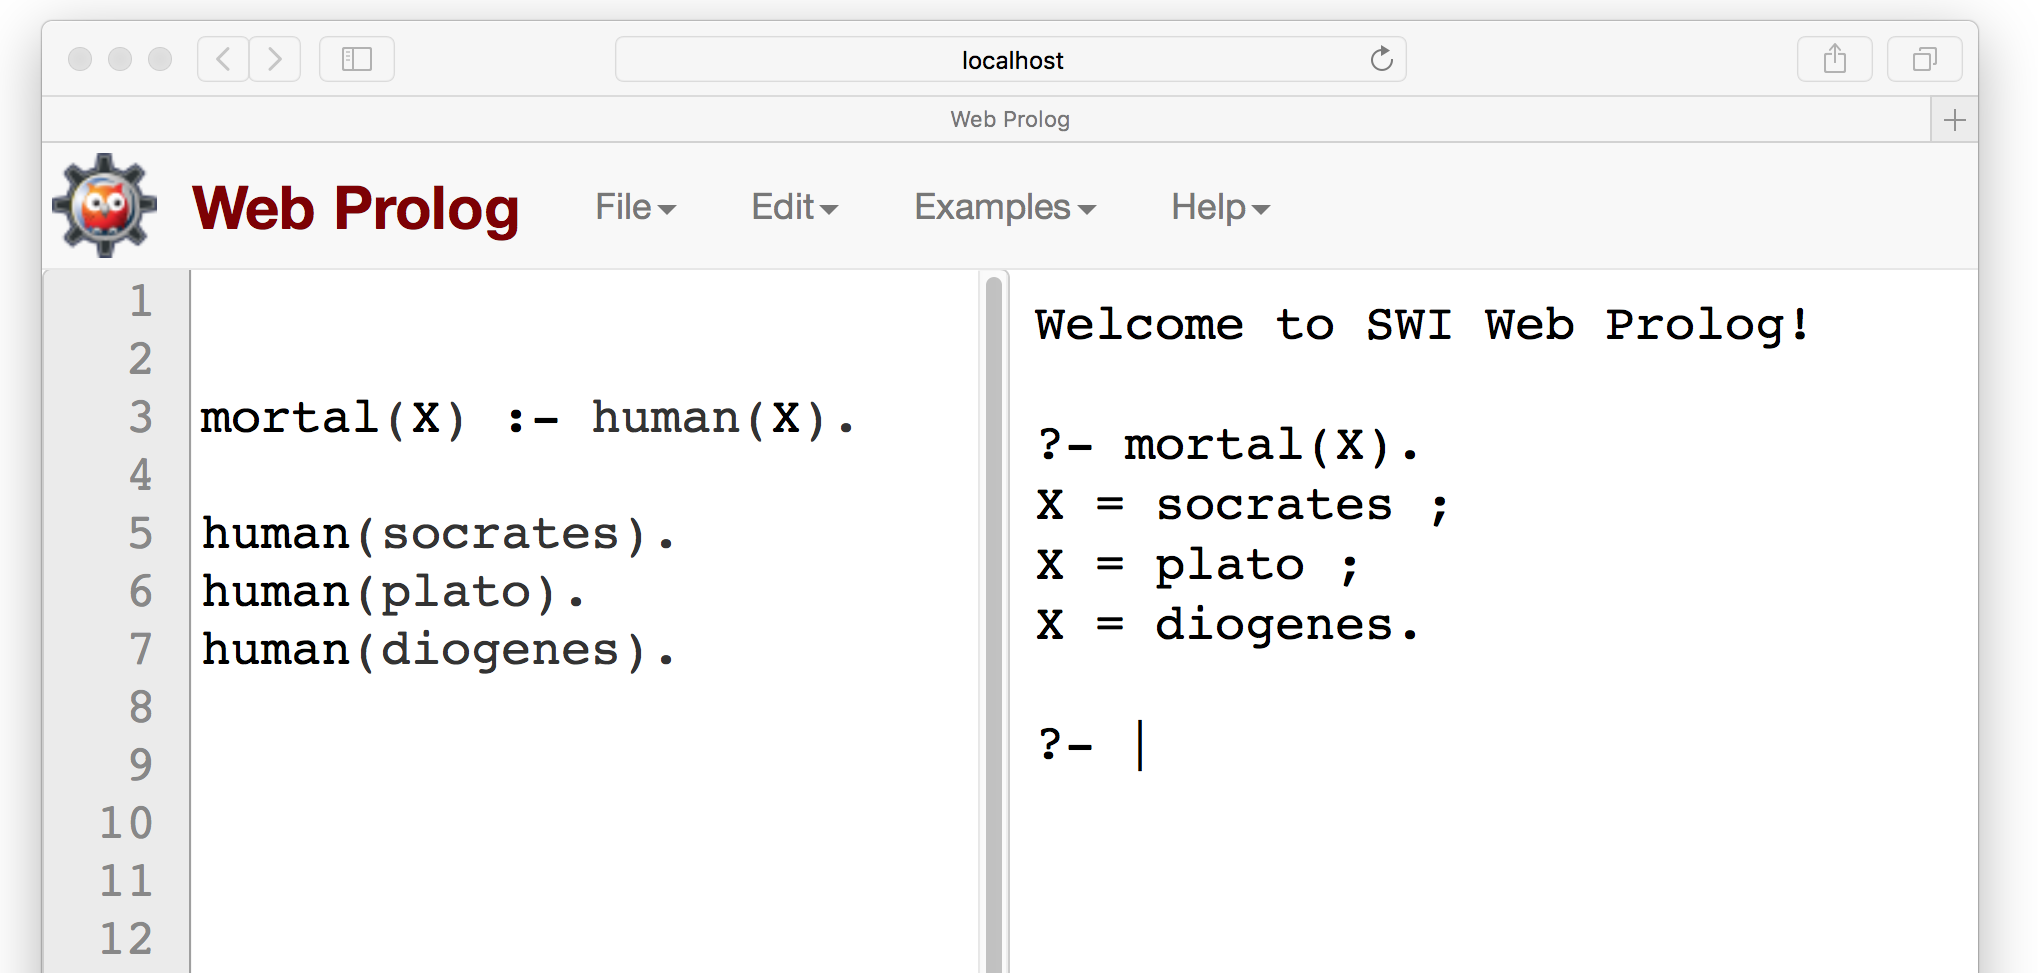
\includegraphics[width=11cm]{swish-2}
    \caption{The proof-of-concept IDE.}
    \label{fig:swish-first}
\end{figure}

\noindent The tiny program shown in the editor can be assumed to have been written by a programmer who has then entered a query in the shell in order to inspect the results produced one-at-a-time in the usual lazy fashion typical of interactions with a Prolog top-level. The scenario, depicted in Figure~\ref{fig:swish-pengine-interaction}, also involves a \textit{node}, identified by the URI \texttt{http://local.org}, to which the IDE has established a connection.

\begin{figure}[h]
    \centering
	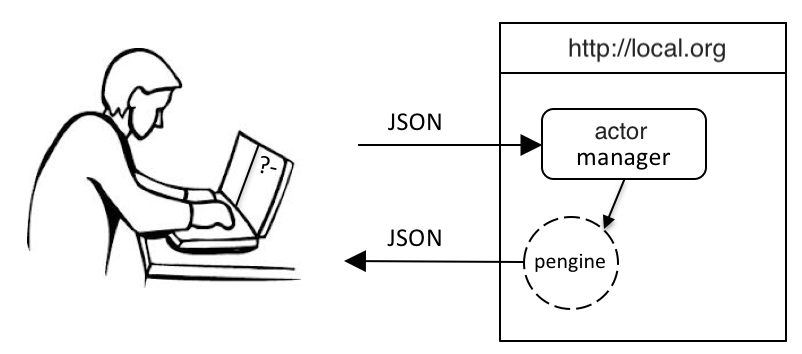
\includegraphics[width=8cm]{swish-pengine-interaction}
    \caption{The shell offers mediated communication between a programmer and a pengine hosted by a node.}
    \label{fig:swish-pengine-interaction}
\end{figure}

A node is an executing Web Prolog runtime environment. Its purpose is to host \textit{pengines} and other actors. A pengine is an actor and a programming abstraction modelled on the interactive top-level of Prolog. It can be seen as a first-class Prolog top-level, accessible from Web Prolog as well as from other programming languages. 

%Should the programmer decide to close or leave the IDE, the pengine with which the shell is connected will be destroyed. (As we shall see, this is related to the Erlang notion of \textit{linking}.)


Despite what Figure~\ref{fig:swish-pengine-interaction} may suggest, the programmer may not be alone in interacting with this particular node. Other programmers may be talking to other pengines running there. They are completely shielded from each other, unless the programs they are running have been written to allow them to communicate. In any case, pengines do not share memory, so in order to share information, they must exchange messages.

A node is equipped with comprehensive web APIs using WebSocket and HTTP as transport protocols, over which a client can run Web Prolog programs defined by the owner of the client, the owner of the node, or by contributions from both. The IDE must be run over the WebSocket protocol.

The task of the node's \textit{actor manager} is to handle the reception of messages sent by clients and arriving over HTTP or WebSocket connections. They may be messages requesting the spawning of a pengine or termination of a pengine, or messages to be forwarded to the pengine addressed by a pid. The actor manager is also responsible for the registration and deregistration of pengines. The registration happens right after the creation of a pengine, deregistration after it has terminated.

Crucially, a node may host a Web Prolog \textit{program} -- a deductive database, an expert system, a digital assistant, a home control system, or another kind of application -- perhaps related to AI and in need of knowledge representation and reasoning. If it does, any pengine running on the node has access to the predicates defined by this program in addition to Web Prolog built-in predicates. The program -- which we shall refer to as the \textit{node-resident} program -- is typically maintained by the owner of the node. Unless programmers are authorised to do so, they are not able to make any changes to it, only the owner is allowed to do so. However, by means of code injection in the workspace of the pengine, programmers are allowed to \textit{complement} the node-resident program with source code that they themselves have written. 

When the programmer enters the URI of the node in the browser's address field, a WebSocket connection is first established between the IDE and the node, and then used to ask the node to spawn a pengine. Messages sent to a node are strings, couched in the syntax of JSON, whereas messages arriving back from a node are expressed in either Prolog or in the JSON format. When talking to a browser, the pengine is instructed to use JSON.


\subsection{The Prolog Web}

\noindent In our first scenario, the programmer was in control of just one single pengine. In other scenarios, this pengine may in turn be in control of and communicate with other pengines and/or other actors. They may be running sequentially, or concurrently. They may be running on the same node, or be distributed over other nodes. That is, in some scenarios, a programmer is in control of the orchestration of what we will refer to as a \textit{multi-actor system}. (Here we exploit the analogy with so called ``multi-agent systems".)

Figure~\ref{fig:swish-pengine-interaction-2} depicts, very sketchily, a situation where a programmer uses the IDE in order to create and control a small system consisting of just three pengines. Another client is querying a forth pengine by means of an HTTP request to the node at \texttt{http://node-2.org}.

%As we have already mentioned, and what will be explained in detail in Chapter~\ref{sec:pengine-profile}, pengines are a kind of actors. What distinguishes pengines from other kinds of actors is the \textit{protocol} they follow when they communicate, i.e. the kind of messages they listen for, the kind of messages they send, and the behaviour this gives rise to. The pengine protocol allows a client to ask queries and a pengine running on a node to respond with answers. All pengines follow this protocol. The shell adheres to it as well, and even a human user of a shell talking to a pengine must adapt to it in order to have a successful interaction with the pengine. 


\begin{figure}[h]
    \centering
	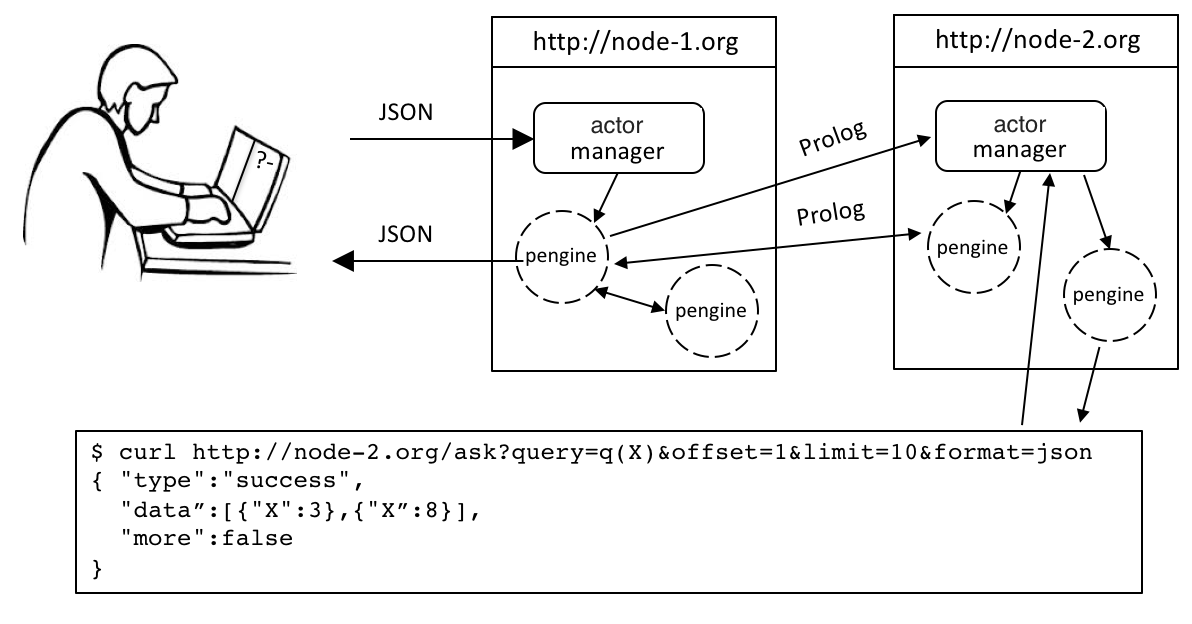
\includegraphics[width=11cm]{swish-pengine-interaction-2}
    \caption{Mediated by the shell, a programmer controls a small \textit{multi-actor system} consisting of just three pengines. Another client is accessing a fourth pengine by means of an HTTP request to the node at \texttt{http://node-2.org}.}
    \label{fig:swish-pengine-interaction-2}
\end{figure}


\subsection{A proof-of-concept demonstrator}

\noindent Our proof-of-concept demonstrator of a Web Prolog node is written in SWI-Prolog \cite{wielemaker:2011:tplp} and can be downloaded from \url{https://github.com/Web-Prolog}, installed and taken for a trial run. The IDE is included in the installation. The demonstrator features an interactive tutorial which provides a tour of the language. The editor and shell supports the usual interactive edit-run cycle and allow users to compose and run their own programs.\footnote{In the future, we intend to use a Web Prolog node as a back-end to SWISH \cite{DBLP:journals/corr/abs-1808-08042}, a much more mature online IDE for Prolog than the one offered by our demonstrator. See \url{https://swish.swi-prolog.org}.}


%The interaction between the shell and the pengine to which the shell is attached uses the \textit{Pengine Communication Protocol} (PCP), implemented as a WebSocket sub-protocol. The protocol will be described in Section~\ref{sec:beyond-erlang}. 

%When the programmer entered the query \texttt{?-mortal(X)}, the shell process sent a message to the node, which forwarded it to the pengine:
%
%\begin{lstlisting}
%connection.send(JSON.stringify({
%  command: 'pengine_ask',
%  pid: pid,
%  query: 'mortal(X)'
%}));
%\end{lstlisting}
%
%\noindent The shell received the following response in return:
%
%\begin{lstlisting}
%{ "type":"success",
%  "pid":"9a343810@http://local.org",
%  "data":[{"X":"socrates"}],
%  "more":true
%}
%\end{lstlisting}
%
%\noindent As a consequence, the shell was updated to show the following:
%
%\begin{lstlisting}
%?- mortal(X).
%X = socrates |
%\end{lstlisting}
%
%\noindent Since the value \texttt{true} of the \texttt{more} property of the JSON message indicated that other solutions to the query existed, a blinking cursor prompted the programmer for input, asking as it were: ``You want more, or not?''. When the programmer responded by typing a semicolon, the shell sent a \texttt{next} message to the pengine and the pengine responded with a new JSON structure representing the second solution to the query \texttt{?-mortal(X)}, and so on.
%
%Messages recognised by the shell fall under different \textit{types}. In addition to the message type that indicates success, there is a type that indicates failure of a query, and a type that indicates errors and other exceptions. Other message types are related to I/O. Would a program call \texttt{read/1} for example, the message that is sent to the shell is of type \texttt{prompt}, and when the programmer enters a term in response to the prompt, an \texttt{input} message is sent to the node and forwarded to the pengine. When the pengine calls the \texttt{writeln/1} predicate, an \texttt{output} message is sent to the shell, which knows exactly what to do with it.


\section{Erlang-Style Programming in Web Prolog}\label{sec:language}

\begin{quote}
Reading the code was fun -- I had to do a double take -- was I reading Erlang or Prolog -- they often look pretty much the same. \flushright \textit{Joe Armstrong} (p.c. June 18, 2018)
\end{quote}


\noindent Erlang is related to Prolog in more than one way. The first implementation was written in Prolog \cite{DBLP:conf/hopl/Armstrong07}, and syntactically they look rather similar and share a lot of terminology. This is something we try to take advantage of when designing Web Prolog and we even name the predicates which support spawning and messaging after Erlang primitives with similar syntax and semantics. However, as we shall see, the primitives for spawning and messaging in Web Prolog are in some ways more expressive than the corresponding Erlang primitives.

As we shall see, we are able to build an architecture for the Prolog Web on top of them in a principled way.

\subsection{Actors}

\noindent Actors, as specified in \cite{DBLP:conf/ijcai/HewittBS73} and \cite{Agha:1986:AMC:7929}, involve entities that have their own mailbox. Communication with and among actors is asynchronous by nature, and actors have location transparency that spans runtimes and machines -- if we have the address to an actor, we can message it. Actors can create new actors, and actors can send messages containing references to other actors. This means that the set of actors forms a graph that can evolve during execution.

\begin{figure}[h]
    \centering
	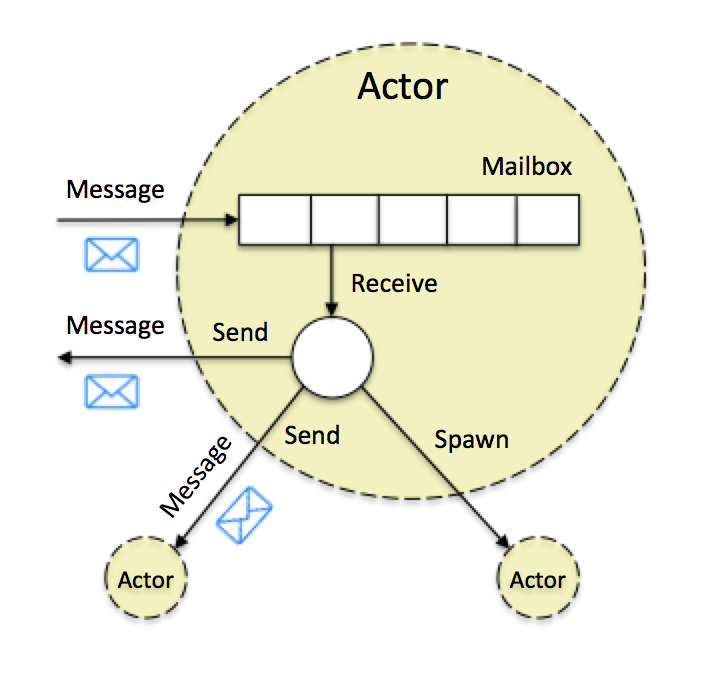
\includegraphics[width=6cm]{actors}
    \caption{An actor}
    \label{fig:actor}
\end{figure}

\noindent Several languages and libraries are branded as actor programming languages, yet the decision to seek inspiration from Erlang (rather than from other actor programming languages such as Akka, Pony, or Elixir) was easy to make. The syntax of Erlang is very close to the syntax of Prolog, and it made sense to take advantage of this when designing Web Prolog. After all, making Erlang programmers feel at home with Web Prolog could turn out to become just as important as making Prolog programmers feel at home with the language.



\subsection{A Simple Count Server}\label{sec:count-server}

\noindent Just like in Erlang, source code which specifies the behaviour of an actor to be spawned can be written in Web Prolog -- the kind of messages it will listen for, and the kind of messages it will send to other actors. Such actors are referred to as \textit{servers} in the Erlang community.

In the editor, a count server can be written as follows and then be loaded by means of injection into the workspace of the pengine to which the shell is attached: 

\begin{lstlisting}
count_server(Count0) :-                 
    receive({             
        count(Pid) ->
            Count is Count0 + 1,    
            Pid ! Count,   
            count_server(Count);
        stop(Pid) ->
            Pid ! stopped(Pid)     
    }).                   
	                      
\end{lstlisting}

\noindent This code contains two primitives foreign to traditional Prolog. The predicate \texttt{receive/1} is used to select and extract messages appearing in the mailbox of the process running the code. The send operator \texttt{!/2} is used to send a message to another process.

The example demonstrates a programming pattern frequently found in Erlang programs and destined to become very useful in Web Prolog as well: a loop is defined where a call to the receive primitive is used to match a message in the mailbox, do something with it, and then continue looping by making a recursive call. The state of the counter is kept in the argument of \texttt{count\_server/1}.

The predicate \texttt{spawn/2-3} is used to create actor processes and it works almost like the spawn function in Erlang. However, while Erlang is a higher-order language in which the spawn function takes an anonymous function as its argument, Prolog (or Web Prolog) is not a higher-order language in this sense. In Web Prolog, \texttt{spawn/2-3} is a \textit{meta predicate} which expects a callable goal to be passed in the first argument. Also, while the spawn function in Erlang exists in more than a dozen variants, Web Prolog has only two, one which takes a list of options and one which relies on their default values. The options are used for the configuration of the actor to be created. Here is how we can spawn the count server from the shell and take it for a trial run:

\begin{lstlisting}
?- spawn(count_server(0), Pid, [
       monitor(true),
       src_predicates([count_server/1])
   ]).
Pid = 891.
?- self(Self).
Self = 324@'http://local.org'.
?- $Pid ! count($Self),
   receive({Count -> true}).
Count = 1.
?- $Pid ! stop($Self).
true.
?- flush.
Shell got stopped(891)
Shell got down(891,true)
true.
?-
\end{lstlisting}

\noindent The \texttt{src\_predicates} option ensured that the count server source code injected into the workspace of the top-level pengine was also injected into the workspace of the spawned server process. Calling \texttt{self/1} determined the identity of the top-level pengine, and \texttt{!/2} was used to send the current count back to the client. Calling the utility predicate \texttt{flush/0} -- also borrowed from Erlang -- allowed us to inspect the content of the top-level mailbox, where a message \texttt{stopped} as well as a \texttt{down} message was found. 

Note also the use of another shell utility feature, borrowed from SWI-Prolog, which allows bindings resulting from the successful execution of a top-level goal to be reused in future top-level goals as \texttt{\$Var}. Together with \texttt{flush/0}, this facility comes in handy during interactive programming in the shell.

In addition to the \texttt{src\_predicates} option, the predicate \texttt{spawn/2-3} supports a number of other options, some of which provide alternative ways to inject source code into the workspace of an actor. Furthermore, the \texttt{node} option allows the programmer to spawn an actor process on a remote node instead of locally, and other options allow the caller to monitor the spawned process or to terminate it should the caller die.


\subsection{Handling Non-determinism}\label{sec:non-det}

%In theory, we should be on the safe side. Sequential Erlang is basically Erlang with its data types, one-way pattern matching, functions and control structures, but without spawn, send, receive, and other constructs designed for concurrent programming. The idea behind Web Prolog can thus be described as an attempt to ``plug out'' the sequential part from Erlang and ``plug in'' sequential Prolog instead. There seems to be no principled reasons why we would not be able to replace the sequential functional language with a sequential relational language, e.g. a logic programming language such as Prolog. Indeed, in \cite{armstrong2003concurrency} Joe Armstrong  writes:
%
%\begin{quote}
%Erlang is a concurrent programming language with a functional core. By this we mean that the most important property of the language is that it is concurrent and that secondly, the sequential part of the language is a functional programming language.
%\end{quote}
%
%\begin{quote}
%The sequential subset of the language expresses what happens from the point it time where a process receives a message to the point in time when it emits a message. From the point of view of an external observer two systems are indistinguishable if they obey the principle of observational equivalence. \textit{From this point of view, it does not matter what family of programming language is used to perform sequential computation.} (Our emphasis.)
%\end{quote}

\noindent Suppose the query given in the argument to \texttt{spawn/2} has several answers, a query such as \texttt{?-human(Who)} for example. Below, a goal containing this query is called, the first solution is sent back to the calling process, and then \texttt{receive/1} is used in order to listen for a message of the form \texttt{next} or \texttt{stop} before terminating:

\begin{lstlisting}
?- self(Self),
   spawn(( human(Who),
           Self ! Who,
           receive({
               next -> fail;
               stop -> true
           })
         ), Pid).
Pid = 940,
Self = 702@'http://local.org'.
?- flush.
Shell got socrates
true.
?- $Pid ! next.
true.
?- flush.
Shell got plato
true.
?- $Pid ! stop.
true.
?-
\end{lstlisting}

\noindent As this session illustrates, the spawned goal generated the solution \texttt{socrates}, sent it to the mailbox of the Prolog top-level and then suspended and waited for messages arriving from the top-level process. When the message \texttt{next} arrived, the forced failure triggered backtracking which generated and sent \texttt{plato} to the mailbox of the top-level shell process. The next message was \texttt{stop}, so the spawned process terminated.

%For an Erlang programmer this particular use of \texttt{receive/1} may come as a surprise. After all, the Prolog concepts of \textit{failure} and \textit{backtracking} and the use of failure to force backtracking are foreign to Erlang. Prolog programmers may recognise a behaviour due to the fact that \texttt{receive/1-2} is a \textit{semi-deterministic} predicate, i.e. a predicate that either fails, or succeeds exactly once. The only way \texttt{receive/1-2} will fail is if the goal in the \textit{body} of one of its receive clauses fails. To see how it pans out in a corner case, consider the following two receive calls:
%
%\begin{lstlisting}
%receive({m(X) -> true})     receive({m(X) -> fail})
%\end{lstlisting} 
%
%\noindent The call on the left will succeed if a message matching the pattern \texttt{m(X)} appears in the mailbox. The call on the right will fail (and possibly cause backtracking) once a message matching the pattern \texttt{m(X)} appears. Only by the left call will the variable \texttt{X} be bound. Both calls will remove the matched message from the mailbox.

The tiny examples in this section highlighted a vital feature of the Web Prolog design as they showed how Prolog-style search and Erlang-style concurrency can be integrated and how a non-deterministic query can be supplied with a deterministic interface. This is precisely the point where the logic programming model and the actor programming model -- represented here by Prolog and Erlang -- interface with each other. This suggests that Prolog's backtracking mechanism is perfectly compatible with, and in fact complements, the proposed Erlang-like mechanisms for spawning actors and handling the communication between them.

The first example above demonstrated an actor adhering to what might be seen as a tiny communication protocol accepting only the messages \texttt{next} and \texttt{stop}. We need to observe, however, that the goal to be solved was hard-coded into the program, and that the program handles neither failure of the spawned goal, nor exceptions thrown by it. There is clearly a need for something more generic. In the next section we will describe the API to a full-blown generic pengine abstraction -- an actor adhering to a considerably more complex protocol.

[FIXME: Refer to Intro to Web Prolog for Erlangers]

\section{Pengines}\label{sec:pengines}

\subsection{A Pengine is an Actor with a Protocol}

\noindent In traditional Prolog the top-level is \textit{lazy} in the sense that new solutions to a query are only computed on demand. However, the top-level is not accessible to programs, i.e. a program cannot \emph{internally} create a top-level, pose queries and request solutions on demand. In Web Prolog, a pengine is a programming abstraction modelled on the interactive top-level of Prolog. A pengine is like a first-class interactive Prolog top-level, accessible from Web Prolog as well as from other programming languages such as JavaScript. 

%We refer to a pengine as an \textit{encapsulated Prolog session}, an abstraction designed to make Prolog programmers feel right at home.

What distinguishes a pengine from other kinds of actors is the \textit{protocol} it follows when it communicates, i.e. the kind of messages it listens for, the kind of messages it sends, and the behaviour this gives rise to. The protocol must not only allow a client to ask queries and a pengine running on a node to respond with answers, it must also allow the pengine to prompt for input or produce output in an order and with a content as dictated by the running Web Prolog program. All pengines follow this protocol. The shell adheres to it as well, and even a human user of a shell talking to a pengine must adapt to it in order to have a successful interaction with the pengine.

The design behind pengines is in fact inspired by the informal communication protocol that we as programmers adhere to when we invoke a Prolog shell from our OS prompt, load a program, submit a query, are presented with a solution (or a failure or an error), type a semicolon in order to ask for more solutions, or hit return to stop. These are ``conversational moves'' that Prolog understands. There are even more such moves, since after having run one query to completion, the programmer can choose to submit another one, and so on. The session does not end until the programmer decides to terminate it. There are only a few moves a client can successfully make when the protocol is in a particular state, and the possibilities can easily be described, by a state machine for example, as we shall do in the next section.


\subsection{The Pengine Communication Protocol}\label{sec:pcp}

%As is often pointed out by Joe Armstrong, message-based systems give us a whole new level of abstraction. In his words, ``We have the black boxes that do things, and we have the messages in between. What goes on inside the black boxes does not really matter; what takes place there is abstracted over.'' This is just as true for pengines and multi-pengine systems as it is for other actors and actor systems. As long as a process delivers correct answers in response to Prolog queries over a Prolog program, it can, for all intents and purposes, be counted as a pengine.

\noindent Figure~\ref{fig:statechart} depicts a statechart specifying the Pengine Communication Protocol (PCP) -- a protocol for the communication between a client and a server (in the Erlang sense of these terms). The server is a pengine running on a node. The client can be any process (including another actor or a JavaScript process) capable of sending the messages and signals in bold to the server. The server is responsible for returning the messages with a leading / back to the client.\footnote{The use of a statechart allows us to show that no matter the current state of the protocol, \textbf{abort} will always take it to the state from which a new query can be asked and \textbf{exit} will always terminate the pengine process.}



%Suppose, for example, that the current state of the protocol is \textbf{s2}, and that the \textbf{abort} signal is received. The transitions leaving \textbf{s2} are tried from the inside and out, and since no label on a transition leaving \textbf{s2} matches, but one placed one step higher in the hierarchy does, a transition to state \textbf{s1} takes place.

\begin{figure}[h]
    \centering
	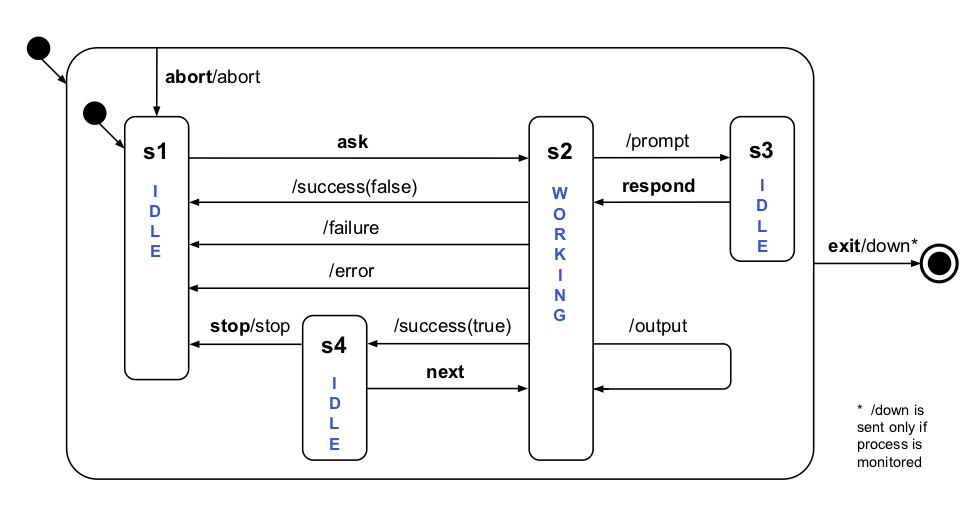
\includegraphics[width=12cm]{statechart}
    \caption{Statechart specifying the PCP for a complete Web Prolog session. The transitions are labeled with \textit{message types}. Types in bold are sent from the client to the pengine, whereas message types with a leading / goes in the opposite direction, from the pengine to the client.}
    \label{fig:statechart}
\end{figure}

Web Prolog comes with a handful of predicates that allows a client to create a pengine and then start talking to it. Most of them will be demonstrated in the next section.


\subsection{In Conversation with a Pengine}

\noindent Below, we show how to create and interact with a pengine process that runs as a child of the current top-level process. %Indeed, what we have here is a pengine running another pengine, a Prolog top-level running another Prolog top-level:

\begin{lstlisting}
?- pengine_spawn(Pid, [
       node('http://ex1.org'),
       src_text("p(a). p(b). p(c)."),
       monitor(true),
       exit(false)
   ]),
   pengine_ask(Pid, p(X), [
       template(X)
   ]).
Pid = 752@'http://ex1.org'.
?- flush.
Shell got success(752@'http://...',[a],true)
true.
?- pengine_next($Pid, [
       limit(2)
   ]),
   receive({Answ -> true}).
Answ = success(752@'http://...',[b,c],false).
?-
\end{lstlisting}

\noindent There is quite a lot going on here. The \texttt{node} option passed to \texttt{pengine\_spawn/2} allowed us to spawn the pengine on a remote node, the \texttt{src\_text} option was used to send along three clauses to be injected into the process, and the \texttt{monitor} options allowed us to monitor it. %These options are all inherited from \texttt{spawn/3}.

Given the pid returned by the \texttt{pengine\_spawn/2} call, we then called \texttt{pengine\_ask/2-3} with the query \texttt{?-p(X)}, and by passing the \texttt{template} option we decided the form of answers. Answers were returned to the mailbox of the calling process (i.e. in this case the mailbox belonging to the pengine running our top-level). We inspected them by calling \texttt{flush/0}. By calling \texttt{pengine\_next/2} with the \texttt{limit} option set to \texttt{2} we then asked for the last two solutions, and this time used \texttt{receive/1} to view them.

Since we passed the option \texttt{exit(false)} to \texttt{pengine\_spawn/2} the pengine is not dead and we can use it to demonstrate how I/O works:

\begin{lstlisting}
?- pengine_ask($Pid, pengine_output(hello)),
   receive({Answer -> true}).
Answer = output(752@'http://ex1.org',hello).
?-
\end{lstlisting}

\noindent We will not show it here, but input can be collected by calling \texttt{pengine\_input/2}, which sends a \texttt{prompt} message to the client which can respond by calling \texttt{pengine\_respond/2}. 

The pengine is still not dead so let us see what happens when a query such as \texttt{?-repeat,fail} is asked:

\begin{lstlisting}
?- pengine_ask($Pid, (repeat, fail)).
true.
?-
\end{lstlisting}

\noindent Although nothing is shown, we can assume that the remote pengine is just wasting CPU cycles to no avail. Fortunately, we can always abort a runaway process by calling \texttt{pengine\_abort/1}:

\begin{lstlisting}
?- pengine_abort($Pid),
   receive({Answer -> true}).
Answer = abort(752@'http://ex1.org').
?-
\end{lstlisting}

\noindent When we are done talking to the pengine we can kill it:

\begin{lstlisting}
?- pengine_exit($Pid, goodbye),
   receive({Answer -> true}).
Answ = down(752@'http://ex1.org',goodbye).
?-
\end{lstlisting}

\noindent Note that messages sent to a pengine will always be handled in the right order even if they arrive in the ``wrong'' order (e.g. \texttt{next} before \texttt{ask}). This is due to the selective receive which defers the handling of them until the PCP protocol permits it. This behaviour guarantees that pengines can be freely ``mixed'' with other pengines or actors. The messages \texttt{abort} and \texttt{exit}, however, will never be deferred.


\subsection{Non-deterministic RPC}\label{sec:ndrpc} 

\noindent For the purpose of a very straightforward approach to the distribution of programs over two or more nodes, Web Prolog offers \texttt{rpc/2-3}, a meta-predicate for making non-deterministic remote procedure calls. Such calls are synchronous and no explicit concurrency is involved, and this makes \texttt{rpc/2-3} remarkably easy to use.

The \texttt{rpc/2} predicate allows a process running in a node A to call and try to solve a query in the Prolog context of another node B, taking advantage of the data and programs being offered by B, just as if they were local to A. A Web Prolog client process queries a node by calling \texttt{rpc/2} with the first argument a URI pointing to the node, and the second argument a query to be run over the predicates offered by the node. Here is a trivial example of its use:

\begin{lstlisting}
?- rpc('http://ex1.org', human(Who)).
Who = socrates ;
Who = plato ;
Who = aristotle.
?-
\end{lstlisting}

\noindent Interestingly, \texttt{rpc/2} retains the logical purity of the predicates it calls, i.e. if the query that is called in the second argument is pure, then the entire call is pure.\footnote{This is a property it shares with the \texttt{call/N} family of Prolog predicates.}

\begin{center}
\textit{Pure Web Prolog = Pure Prolog + \texttt{rpc/2-3}}
\end{center}

\noindent The union of all partitions of the Prolog Web which are written in pure Web Prolog forms what we think of as the \textit{pure Prolog Web}. With a large number of nodes running pure Web Prolog programs interlinked to other pure Web Prolog programs, we may \textit{in theory} be able to create a Web of Logic on top of the conventional Web, a layer that can \textit{in principle} grow as big as we want it to grow, and even into a network spanning the whole globe, just like the conventional web has done, while still adhering to the formal (model or proof theoretic) semantics of the pure subset of the Prolog language. In practice, this may never happen, but the \textit{architecture} is there. 

Even in scenarios where a portion of the Prolog Web is pure, it often makes sense to regard each node as a kind of agent, and to treat the Web Prolog code held by the node as the \textit{beliefs} of this agent. Thinking about programs in this way, which is really only possible when programs are declarative, suggests that \texttt{rpc/2} can be treated as a higher-order \textit{epistemic operator} where a call such as \texttt{rpc(URI,Q)} is actually asking whether the pengine at \texttt{URI} \textit{believes} that \texttt{Q}. Thus, a clause such as

\begin{lstlisting}
mortal(X) :- rpc('http://ex1.org', human(X)).
\end{lstlisting}

\noindent can, in the syntax of predicate logic enhanced with a higher-order predicate \textit{believes/2}, be formulated as

\begin{center}
$\forall x [believes(ex_1, human(x)) \rightarrow mortal(x)]$
\end{center}

\noindent Thinking about it in this way, it makes perfect sense to say that one node believes that \texttt{human(plato)} is true, while another node does not:

\begin{lstlisting}
?- rpc('http://ex1.org', human(plato)).
true.
?- rpc('http://ex2.org', human(plato)).
false.
?-
\end{lstlisting}

\noindent The following query simply asks whether the nodes \texttt{http://ex3.org} and \texttt{http://ex4.org} \textit{agree} that \texttt{p(X)}:

\begin{lstlisting}
?- rpc('http://ex3.org', p(X)), 
   rpc('http://ex4.org', p(X)).
X = 1 ;
X = 2.
?-
\end{lstlisting}

\noindent Two nodes may hold contradictory beliefs, and sometimes this can be detected: 

\begin{lstlisting}
?- rpc('http://ex5.org', square(Item)), 
   rpc('http://ex6.org', circle(Item)).
Item = a132.
?-
\end{lstlisting}


\noindent We do not have to go as far as to define a special epistemic operator, however. Another way to understand what is going on here is to realise that any realistic knowledge representation language needs an explicit construct for specifying the \textit{scope} or the \textit{context} of the inference -- the knowledge base with respect to which inference is to be made. As used in \texttt{rpc/2-3}, the humble URI can be seen as a way to indicate such a scope. As argued by \cite{Kifer2005}, scoped inference is in fact mandatory for realising Negation As Failure (NAF) on the Web, because to apply any form of the closed world assumption, one needs to know the entire knowledge base first, something which is not really possible for the Web since its boundaries cannot be clearly delineated.

\subsection{An Implementation of rpc/2-3}\label{sec:rpc-implementation}

\noindent Below, we show an implementation of \texttt{rpc/2-3} which is built on top of a pengine spawned on a remote node and a local loop that waits for answers arriving from it:

%This section looks at an implementation of \texttt{rpc/2-3} with code clean enough to nail down its semantics. The implementation is built on top of a pengine spawned on a remote node and a local loop that waits for answers. %From this point on the communication is synchronous:

\begin{lstlisting}
rpc(URI, Query, Options) :-
    pengine_spawn(Pid, [
         node(URI),
         exit(true),
         monitor(false)
       | Options
    ]),
    pengine_ask(Pid, Query, Options),
    wait_answer(Query, Pid).
\end{lstlisting}

\begin{lstlisting}
wait_answer(Query, Pid) :-
    receive({
        failure(Pid) -> fail;            
        error(Pid, Exception) -> 
            throw(Exception);                  
        success(Pid, Solutions, true) -> 
            (   member(Query, Solutions)
            ;   pengine_next(Pid), 
                wait_answer(Query, Pid)
            );
        success(Pid, Solutions, false) -> 
            member(Query, Solutions)
    }).
\end{lstlisting}

\noindent Note how the disjunction in the body of the third receive clause and the use of \texttt{member/2} in the third and fourth clauses turn the deterministic calls made by \texttt{pengine\_ask/3} and \texttt{pengine\_next/1} into the expected non-deterministic behaviour of \texttt{rpc/2-3}. 

It may be helpful to think of what is going on here as a very simple kind of \textit{buffering}, and in particlar as the use of what is usually referred to as a \textit{bounded buffer}. The value of the \texttt{limit} option represents the size of the buffer. The producer (i.e. the remote pengine process) is allowed to get ahead of the consumer (i.e. the process running the \texttt{rpc/3} call), but only until the buffer is full. The consumer can take elements from the buffer immediately without waiting. When the buffer is empty, the producer is prompted to produce more elements, until the buffer is full. In our proof-of-concept implementation, the consumer and the producer are not running concurrently (as they do not execute different tasks during overlapping periods of time). A possible optimisation would be to allow them to do so by letting the remote process compute additional solutions while waiting for a \texttt{next} message and return all available solutions if it arrives. If a \texttt{stop} message arrives instead, or if time has run out, the additional solutions would be discarded. Note that nothing here concerns the client, as it is the owner of the node who would need to enable this optimisation.

This implementation is clean enough to nail down the semantics of \texttt{rpc/2-3}, but it only works over a WebSocket connection. However, it turns out that a version of \texttt{rpc/2-3} with the exact same semantics can instead be implemented on top of the stateless HTTP described in Section~\ref{sec:browser}. This implementation is more complex, so we do not show it here.

\subsection{Reducing the Number of Network Roundtrips}\label{sec:reducing-roundtrips}

\noindent When \texttt{rpc/2} is used, some of the backtracking involved in the search for solutions is taking place over the network, and network roundtrips take time -- a lot of time in comparison with other computational steps programs typically perform. Since calling a remote program may involve very many roundtrips during backtracking, the times may add up to a significant slowdown compared to making a local call. By passing the \texttt{limit} option to \texttt{rpc/3} we can make the communication less ``chatty'' and avoid many roundtrips. Here is an example:

\begin{lstlisting}
?- rpc('http://ex1.org', human(Who),[
       limit(10)
   ]).
Who = socrates ;
Who = plato ;
Who = aristotle.
?-
\end{lstlisting}

\noindent As the example tries to convey, the behaviour of the call, as seen from the point of view of the client, does not change. After having been presented with the first solution to the query the programmer still needs to type a semicolon in order to see the next solution. But under the hood, the next solution has already been computed and returned to the client as the second member of a list containing all three solutions. Thus no new request to the node needs to be made. So while the retrieval of the three solutions to the query required three network roundtrips before we applied the option, it will now only require one roundtrip. More generally, a query with $n$ solutions would (normally and by default) require $n$ roundtrips if we wanted to see them all, but if we set \texttt{limit} to $i$, the same query would only require $n/i$ roundtrips, or just one roundtrip if $n/i < 1$.

Use of the \texttt{limit} option is fine also from a purity point of view -- it has nothing to do with logic and the declarative reading of the query, but must be treated as a \textit{pragma} -- as a language construct that specifies the granularity with which the conversation between the client and the node should be conducted. Passing the option \texttt{limit(10)} can be understood as saying: ``Send me the answers in chunks of \texttt{10}. I will be looking at them one-by-one, but I want them in batches.'' Although adding the limit pragma to a query will have no effect on the meaning of the query, it can have a significant effect on performance when running the query over a cluster of nodes.


\subsection{Shuffling Code and Data Back and Forth}

\noindent On the internet, the cost of shuffling code and data back and forth across remote boundaries is significant, yet cannot be avoided. But in which direction should the shuffling be made in order to bring down the cost? The answer is most likely that it varies and that programmers should be given a choice.

%It is often more efficient to bring a few lines of code to the data rather than moving an often large amount of data to the code. In the case of data being frequently updated (think stock market data for example) the gain is probably significant. On the other hand, if the data is more or less static (think geo-political data for example) and we want to query it a lot, then bringing the data to the code may be more efficient.

The obvious way to bring code to the data in Web Prolog is to inject source code into the remote process created by \texttt{rpc/2-3}. With the following call, we do just that:

\begin{lstlisting}
rpc('http://ex1.org', foo(X), [
    src_text("mortal(X) :- human(X).")
])
\end{lstlisting}

\noindent In combination with the \texttt{src\_uri} option \texttt{rpc/3} can also be used to bring the data to the code. Here is an example:


\begin{lstlisting}
rpc(localnode, human(X), [
    src_uri('http://ex1.org/src')
])
\end{lstlisting}

\noindent The source held by the node at \texttt{http://ex1.org} is injected into the workspace of the underlying pengine before the query \texttt{?-human(X)} is tried, thus isolation is provided.

These two examples suggest a useful symmetry which allows Web Prolog code to flow in either direction, from the client to the node or from the node to the client. The choice is determined by the programmer's selection of options configuring the actor to be spawned, but it can in principle also be decided programmatically at runtime.

%When discussing the bringing of ``code to the data'' versus ``data to the code'', it is important to keep in mind that the distinction between code and data is not as sharp in Prolog as it is in most other programming languages.


\section{The Web APIs}

\subsection{The WebSocket API}



\subsection{The HTTP API}

\noindent An IDE for traditional Prolog is a fairly demanding type of web application. Although the conversation between the programmer and the pengine must always be initiated by the programmer using the shell, the interaction may at any point turn into a mixed-initiative conversation driven by requests for input made by a running query. What makes unconstrained mixed-initiative interaction feasible is the support for efficient bi-directional messaging offered by a node thanks to the use of the WebSocket protocol.

Other kinds of web applications may have no need for mixed-initiative interaction. In order to serve such applications, a Web Prolog node offers a stateless HTTP API. Interestingly, it also turns out that since \texttt{rpc/2-3} does not produce output or request input, it can be run over HTTP instead of over the WebSocket protocol. In our proof-of-concept implementation this is the default transport.

In order to serve \texttt{rpc/2-3}, a Web Prolog node offers a stateless HTTP API. To retrieve the first solution to \texttt{?-human(X)} using this API, a GET request can be made with the following URI:

\begin{lstlisting}
http://ex1.org/ask?query=human(X)&offset=0 
\end{lstlisting}

\noindent Here too, responses are returned as Prolog or as Prolog variable bindings encoded as JSON. Such URIs are simple, they are meaningful, they are declarative, they can be bookmarked, and when the GET method is used, responses are cachable by intermediates. 

In order to ask for the second and third solution to \texttt{?-human(X)}, another GET request can be made with the same query, but setting \texttt{offset} to \texttt{1} this time and adding a parameter \texttt{limit=2}. To avoid recomputation of previous solutions, the actor manager keeps a pool of active pengines. For example, when the actor manager received the first request it spawned a pengine which found and returned the solution to the client. This pengine -- still running -- was then stored in the pool where it was indexed on the combination of the query and an integer indicating the number of solutions produced so far (i.e. \texttt{1} in this case). When a request for the second and third solution arrived, the actor manager picked a matching pooled pengine, used it to compute the solutions, and returned them to the client. Note that the second request could have come from any client, not necessarily from the one that requested the first solution. This is what makes the HTTP API stateless.

The maximum size of the pool is determined by the node's settings. To ensure that the load on the node is kept within limits, the oldest active pengines are terminated and removed from the pool when the maximum size is reached. This \textit{may} mean that some solutions to some subsequent calls must be disposed of, but this will not hurt the general performance.



\section{Prolog Web $\approx$ Semantic Web?}\label{sec:wp-ws-sw}

\noindent The conventional web, already in its most primitive form as a Web of Documents (also known as Web 1.0), is \textit{distributed} (running on more than one machine), \textit{decentralised} (running at different geographical locations and/or having different owners) and \textit{open} (anyone can use and contribute). These are some of the traits the Prolog Web inherits from the conventional web. Since the Pure Prolog Web adds logic and reasoning to the conventional web, we appear to be approaching something resembling the \textit{Semantic Web}, a vision of a machine readable web first proposed in May 2001 in an article by Tim Berners-Lee, James Hendler and Ora Lassila published by Scientific American \cite{bernerslee2001semantic}. The gist of this article is captured by the following three quotes:

\begin{quote}
The Semantic Web is an extension of the current web in which information is given well-defined meaning, better enabling computers and people to work in cooperation.
\end{quote}

\begin{quote}
For the semantic web to function, computers must have access to structured collections of information and sets of inference rules that they can use to conduct automated reasoning.
\end{quote}

\begin{quote}
Adding logic to the Web -- the means to use rules to make inferences, choose courses of action and answer questions -- is the task before the Semantic Web community at the moment.
\end{quote}

\noindent Surely, words and phrases such as ``logic'', ``automated reasoning'', ``answer questions'' remind us about what Prolog is good at, and clearly, the phrase ``an extension of the current web'' is a description that also fits the Prolog Web. This prompts us to investigate whether the Prolog Web might serve as a ``poor man's'' semantic web, and whether it -- for some use cases -- might even be a better choice of technology.

There has been a lot of activity in the Semantic Web field in the years following the publication of \cite{bernerslee2001semantic}. The Semantic Web vision is many-faceted and has prompted research and development in many areas of computer science. A plethora of languages for knowledge representation and querying have been designed and some of them have been standardised by the W3C. They are web logic languages, rather than programming languages. Components such as reasoners, web services, service discovery facilities, user interface frameworks, agent platforms and other forms of infrastructure for the Semantic Web have also been designed and prototyped but not yet standardised. 

As such, the ideas behind the Semantic Web may be both sound and powerful, but the W3C recommendations are complex, and it is often difficult to see how they fit together and how to make use of them when building practical applications.\footnote{This has caused some to give up on the Semantic Web. See \url{http://inamidst.com/whits/2008/ditching} and \url{https://www.linkedin.com/pulse/why-semantic-web-has-failed-kurt-cagle}} The Prolog Web is much simpler, and we might ask ourselves if it could, in at least some cases, serve as an easier to use replacement for the Semantic Web. Unfortunately, for some Semantic Web use cases, we are not quite there yet. While logic, automated reasoning, openness and decentralisation may be necessary ingredients in a truly semantic web, they surely are not sufficient. 


\subsection{To have the cake and eat it too}\label{sec:have-the-cake}

\noindent The architecture of the Semantic Web is layered, one layer of languages above another, where each layer exploits the capabilities of the layers below. The layers at the bottom serve also the conventional web. A commonly used illustration of this idea is the so called ``Semantic Web Layer Cake'', one variant of which is depicted in Figure~\ref{fig:cake}.

\begin{figure}[h]
    \centering
	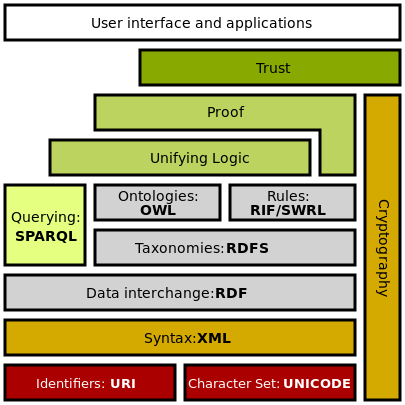
\includegraphics[width=6cm]{cake}
    \caption{The Semantic Web Layer Cake}
    \label{fig:cake}
\end{figure}

\noindent A diagram of this kind can only give us a vague and somewhat impressionistic view of what the Semantic Web involves, but can at least be used to lend structure to a comparison with the Prolog Web. Starting from the bottom of the ``cake'', the Uniform Resource Identifier (URI) has played an important part in the development of the Web already from its inception, at first only as a way to locate a document, but on the Semantic Web it can be used to name anything. The Prolog Web, as described so far, may use it in this latter way too, but also to locate programs as well as to uniquely identify answers to queries. Not surprisingly, URIs are normally represented as \textit{atoms} in Web Prolog, and since Web Prolog is a fairly general programming language, it is of course easy to pick them apart and access their components, or to build new URIs from arbitrary components.\footnote{As it seems independently useful, we may want to introduce the namespace mechanism available in Cliopatria in all Web Prolog profiles. }

Unicode, another necessary part of the conventional Web, may also be seen as a naming mechanism, as it aims to uniquely identify all the characters in all the written languages of the world. Support for Unicode is increasing throughout the world of computing, as the benefits of one common character set are overwhelming when programs are used in a global environment such as the Web. Not all Prolog systems are capable of working with Unicode, but it seems clear that a world wide Web Prolog has to be.

The Semantic Web cake usually has a layer indicating a reliance on XML, seen as the syntax of the Semantic Web. In the context of the Prolog Web we wish to somewhat downplay the importance of XML in favour of the Prolog \textit{term} data structure and the JSON format. Our impression is that most researchers would agree that XML is not fundamental to the Semantic Web but should rather be viewed as a \textit{data interchange format} (and, in fact, one out of many). A particular Prolog Web node may well be able to parse and generate XML documents, but a node is not strictly required to be able to do so. 


\subsection{Semantics proper}\label{sec:semantics-proper}

\noindent Above the XML layer of the Semantic Web cake we find the layers devoted to semantics proper, where RDF lays the very foundation. From a Prolog point of view, RDF is a predicate with three arguments.

ClioPatria is an RDF-application development framework developed by Wielemaker et al and built on top of SWI-Prolog \cite{wielemaker2016cliopatria}. The Cliopatria white paper describes the benefits as follows:\footnote{\url{http://cliopatria.swi-prolog.org/help/whitepaper.html}} 

\begin{itemize}

\item The single primitive \texttt{rdf(S,P,O)} suffices to realise all the basic graph-pattern matching that can be done in SPARQL.

\item We can give a name to a query and build complex queries from simple ones. This greatly simplifies maintenance of complex queries.

\item Optimisation and unfolding can be used to achieve optimal performance at a small cost.

\item Instead of the predefined SPARQL functions and conditions, we can apply any Prolog predicate as a condition or function anywhere in the query. We can also introduce other relations (e.g., from an RDBMS) into our predicates.

\item The RDF store is tightly connected to Prolog. This allows for arbitrary reasoning with and exploration of the RDF graph at low cost.

\end{itemize}

\noindent To our knowledge, no other general-purpose programming language besides Prolog is capable of providing such a clean interface to RDF. We would even encourage the view of the syntaxes of the different RDF serialisation formats as variants of the syntax of (a subset of) Prolog. Here we give an example of triples represented in Prolog taken from the RDF 1.1 primer document:\footnote{\url{http://www.w3.org/TR/2014/NOTE-rdf11-primer-20140624/\#section-n-triples}}

\begin{lstlisting}
rdf('http://example.org/bob#me',
    'http://...rdf-syntax-ns#type',
    'http://xmlns.com/foaf/0.1/Person').
rdf('http://example.org/bob#me',
    'http://xmlns.com/foaf/0.1/knows',
    'http://example.org/alice#me').
rdf('http://example.org/bob#me',
    'http://schema.org/birthDate',
    literal(type('http://...#date',
                 '1990-07-04'))).
\end{lstlisting}

\noindent Like SPARQL and Turtle, the Prolog RDF layer allows for prefix notation. Prefixes are declared using \texttt{rdf\_register\_prefix(Prefix,URI)}, after which URIs can be written as \texttt{prefix:localname}. We will use this notation from here on, using the conventional prefixes as defined on \texttt{http://prefix.cc/}. Given an RDF database, Prolog allows us to write graph patterns as they appear in e.g., SPARQL as a conjunction of \texttt{rdf/3} relations. For example to get the birth dates of people somebody knows we can write:

\begin{lstlisting}
known_with_birthdate(Me, He, Date):-
    rdf(Me, foaf:knows, He),
    rdf(He, schema:birthDate, Date).
\end{lstlisting}

\noindent The \texttt{known\_with\_birthdate/3} version in Prolog has many advantages over the SPARQL version, which we will explain below. First, because the Prolog version has an explicit name, it is easy to reuse it in other queries. This allows developers to incrementally build more sophisticated functionality on top of existing, proven and tested building blocks. This is an effective way to avoid the large and complex SPARQL queries often found in other Semantic Web applications. A second advantage is that the three arguments to \texttt{known\_with\_birthdate/3} can be used both to query and to filter. [FIXME: I've probably stolen some text here from Jan et al.]

The interactive session below illustrates the use of \texttt{known\_with\_birthdate/3} to query the triple store:

\begin{lstlisting}
?- known_with_birthdate(Me, He, Date).
Me = 'http://example.org/bob#me'
He = 'http://example.org/alice#me'
Date = literal(type(xsd:date,'1990-07-04') ;
Me = 'http://example.org/bob#me'
He = 'http://example.org/john#me'
Date = literal(type(xsd:date,'1992-09-06') ;
...
\end{lstlisting}

\noindent The following quote wraps up the position taken by Wielemaker and his team, a position that we subscribe to:

\begin{quote}
We do not consider SPARQL adequate for creating rich semantic web applications. SPARQL often needs additional application logic that is located near the data to provide a task-specific API that drives the user interface. Locating this logic near the data is required to avoid protocol and latency overhead. RDF-based application logic is a perfect match for Prolog and the RDF data is much easier queried through the Prolog RDF libraries than through SPARQL.
\end{quote}

\noindent We leave the work by Wielemaker and his team here with a note that we probably have not made it full justice, and with the advice to interested parties to read \cite{wielemaker2016cliopatria}.


---

Triples serve as a universal representation of relations, and through the process of reification the ``subject predicate object'' schema can in principle capture all the kinds of relations we might want to represent, but it can often become unwieldy. It is often better to generalise from these 3-tuples to n-tuples, and this is supported by the Prolog Web.

---

Making our way up the layers of the cake, we find OWL. Based on description logics, a subset of predicate logic only partly overlapping with the Horn clause logic subset, OWL is used for establishing the fixed, controlled ontology vocabularies deemed so important for the Semantic Web. The Prolog Web lacks the concept of ontologies. It is not that we cannot build ontologies in pure Web Prolog. We can, but due to the less expressive Horn clause logic they will less useful. While so called ISA hierarchies can easily be represented -- already \cite{deliyanni1979logic} demonstrated this -- features such as range restrictions \textit{et cetera} are more problematic. (Since Web Prolog is a general-purpose programming language, we can of course use it to write programs capable of reasoning with (say) OWL, but this is a different matter.)

Again, there appears to be a common understanding now in the Semantic Web community that the word ``Semantic'' as in ``Semantic Web'' is a little over ambitious and evokes the wrong expectations. For the baseline functionality and majority of use cases, ontologies may not be needed. 

Having said that, we need to take the distinction between \textit{syntactic interoperability} and \textit{semantic interoperability} into account. Semantic interoperability is (according to Wikipedia) ``the ability of a computer system to exchange data with unambiguous, shared meaning, and is seen as a requirement to enable machine computable logic, inferencing, knowledge discovery, and data federation between information systems.'' Syntactic interoperability cannot provide us with this. [FIXME: This must be integrated in a better way.]

One thing to notice here is that the Semantic Web community makes a clear distinction between knowledge representation languages (such as RDF, RDFS and OWL) and query languages (such as SPARQL), Prolog (including Web Prolog) can, at least to some extent, fill both of these roles. Granted, as a knowledge representation language, Prolog is not very expressive -- there are a lot of things we simply cannot say in Horn clause logic, and there are certainly queries that cannot be asked in Prolog used as a query language. However, the point is that the \textit{same} language can be used for \textit{both} knowledge representation and querying. This is a unique and very valuable feature of Prolog, not shared by any other (major) programming language. 


\subsection{Proof and trust}\label{sec:proof-and-trust}

\noindent The Semantic Web community does not have much to say about the cake layers labelled Proof and Trust, and neither have we. Recall, however, that as one way to increase (one particular kind of) trust in a Web Prolog code resource, we can at least generate \textit{proof trees}, and we have already demonstrated one way of doing this in Section~\ref{sec:rpc-and-proofs}. 

As an example of a more interesting use of \texttt{rpc/2-3} and code injection we suggest a way to generate a \textit{proof tree} for a query using rules that may call \texttt{rpc/2}. The idea is to use a proof constructing meta-interpreter that injects \emph{itself} in the pengine running the call to \texttt{rpc/3}. (Look carefully at the second clause of \texttt{prove/2} below.) With this program it is possible to generate a proof tree for any query (involving the subset of Web Prolog the meta-interpreter can handle), even those that need access to another node to be answered (and which in turn may need yet another node, and so on).


\begin{lstlisting}
prove(true, true) :- !.
prove(rpc(URI, Bs), node(Node, BSProof)) :- !,
    rpc(URI, prove(Bs, node(Label, BSProof)), [
        src_predicates([prove/2, prove_body/2])
    ]),
    atomic_list_concat([Label, URI], '@', Node).
prove(H, node(Node, BSProof)) :-
    clause(H, Bs),
    prove_body(Bs, BSProof),
    term_to_atom(H, Node).

prove_body((B, Bs), [BT|BTs]) :- !,
    prove(B, BT),
    prove_body(Bs, BTs).
prove_body(B, [BT]) :-
    prove(B, BT).
\end{lstlisting}

\noindent Note the use of the \texttt{rpc/3} option \texttt{src\_predicates(List)}. It sends the local predicates denoted by
\texttt{List} to the underlying remote pengine, where \texttt{List} is a list of predicate indicators. 

A common criticism against such proofs is that they tend to grow too big and detailed. In some domains this may be true, but in other domains it would probably work to the satisfaction of its users. Besides, a very similar approach might hide what is going on inside a node, and only show the bigger picture.  

The above meta-interpreter is likely to blow up for scenarios involving very large proof trees. This is not really a problem since the suggestion is not to make \texttt{prove/2} a builtin predicate. It is the author of the client code who decides what kind of proofs should be built and how, and it is this author's responsibility to write a version of a proof collector predicate that works for a given scenario. 

In practice we probably do not want to show the proof at the clause level. The approach may however also be useful for showing the distribution of the query solving work over multiple nodes. Such a distribution can also be rendered as a tree. In order to avoid including clause level proofs, we need to replace the third clause of \texttt{prove/2} with:

\begin{lstlisting}
prove(H, Proof) :-
    clause(H, Bs),
    prove_body(Bs, Proof).
\end{lstlisting}

\noindent If we make this change we are no longer building proofs, so to better fit its purpose, we should probably change the name of the predicate as well.

Furthermore, we would like to suggest that the notion of trust can be interpreted in a very mundane way, where one way to build and maintain trust in a Web Prolog resource is to offer a way to inspect the Web Prolog code stored on the remote node in question, e.g. through a browsing or listing facility. It goes without saying that the use of good predicate names and good variable names is also, as always, important. Finally, we must not forget the role of good documentation.


\subsection{Cakes and towers}\label{sec:other-cakes}

\noindent As we have already indicated, many variants of the Semantic Web layer cake have been put forward. It appears that some variants are more in line with the theory behind logic programming than others. The two-tower architecture of \cite{Horrocks2005} depicted in Figure~\ref{fig:cake-hendler} presents two possible instantiations of the Semantic Web layered architecture. 

\begin{figure}[h]
    \centering
	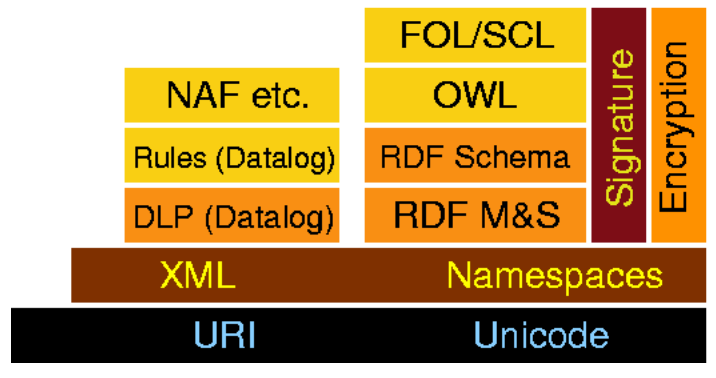
\includegraphics[width=6cm]{cake-hendler}
    \caption{The Two-Tower Semantic Web Layer Cake}
    \label{fig:cake-hendler}
\end{figure}

\noindent The tower to the right basically captures the same idea as the cake in Figure~\ref{fig:cake}. The tower to the left is different, and is more firmly grounded in the logic programming paradigm proper. Here DLP stands for Description Logic Programs, a subset of First Order Logic which includes the Datalog fragment, but which also has some of the expressive power found in OWL, useful for building ontologies. On top of DLP, rules can be formulated and extended with Negation As Failure (NAF) etc. The ``etc'' here is significant as it indicates other possible extensions of the Horn clause fragment, and in the world of logic programming research there are indeed a lot of those around. In the same spirit as the Two Tower paper, \cite{Kifer2005} argue that a realistic architecture for the Semantic Web must be based on multiple independent, but interoperable, stacks of languages, and they put special emphasis on a stack similar to the tower to the left in Figure~\ref{fig:cake-hendler}, arguably closer to logic programming than the tower to the right.

It would be interesting to see if the Prolog Web could be developed into a Logic Programming Web more generally. A point often raised is that the large and open world of the Web will almost certainly need some forms of uncertainty and fuzziness. Perhaps the implementation of ProbLog (in Java) can be extended into a node capable of answering  queries in a Web Prolog compatible way, thus providing probabilistic logic programming.  [FIXME: Add reference to Datalog and cplint + Something about Well-Founded Semantics.]


As regards the relation of Web Prolog to the two towers, we can think of it in either of two ways: Web Prolog can be seen as an instantiation of the tower on the left, except that it is not based on XML and that it needs to come with tabling, or it can be regarded as a third tower. The programming language capabilities of Web Prolog indicates that the latter may be preferred.


\subsection{Prolog Web reasoning engines}\label{sec:prolog-web-reasoners}

\noindent The Semantic Web community usually makes a distinction between Semantic Web \textit{languages} and Semantic Web \textit{reasoning engines} (or just ``reasoners"). This distinction makes a lot of sense, especially since different reasoners can be used for the same language. The distinction can of course be made for Web Prolog too. Any machinery for computing with the pure subset of Web Prolog may well be seen as a \textit{Prolog Web reasoner}. Indeed, the humble pengine should be viewed as a reasoning engine for the Prolog Web, although it is not only that, but an \textit{interaction engine} as well, taking care of the necessary communication with other processes through what from a logically pure view must be deemed side effects.

As we have argued already, logic and protocol form two separate aspects of Prolog. Given the abstractness of the protocol (cf. Section~\ref{sec:protocol-properties}) it should be expected that it can be given a concrete manifestation not only for Prolog but also for other logic programming languages, and not only for pengines, but also for other reasoning engines.

Recall that since general I/O is non-pure, the only communication possible with a pengine running a pure Web Prolog program is the sending of queries and the reception of answers the pengine is sending back in response. This is a restricted form of I/O.

There are several possibilities here. One is to keep the restricted communication capabilities of a pengine, but to strengthen its reasoning abilities. This can be done without introducing more language features; adding the ability to do \textit{abduction} in Horn clause theories would be one example. Using less expressive languages still compatible with Prolog is of course also possible. Datalog is one example. Datalog reasoners (based on e.g. the magic sets algorithm) have properties that are interesting in certain use cases. The communication with such reasoners can be done over the Pengine Communication Protocol, and in fact over a subset of it. [FIXME: Elaborate this. Will it always work?]


\subsection{Prolog Web Services and Service Discovery}\label{sec:semantic-web-services}

\noindent \textit{Semantic Web Services}, like conventional web services, are the server end of a client-server system for machine-to-machine interaction via the Web. As we have already seen, the approach we take with the Prolog Web is to specify a set of generic web service APIs that covers everything a web logic programmer could possibly ask for.

Web Prolog nodes are designed to serve not only the front-ends of our applications but also to be part of an ecology -- a section of the Prolog Web. This means exposing our data and programs to others, to be queried and copied and integrated, often even without our explicit consent or even our knowledge. Others are thus invited to use our APIs and to treat our node as just another part of the Web's infrastructure, as a world-wide assortment of Web Prolog predicates to call in order to get things done.

In contrast to the Semantic Web, the so called \textit{Programmable Web} has made its mark in a big way.\footnote{\textit{ProgrammableWeb} is also the name of a website that publishes a repository of web APIs and has documented over 17,000 open web APIs. See \url{https://www.programmableweb.com/category/all/apis}. } Users expect web applications to call out to third-party services as necessary in order to better serve them, and web application developers are no longer content with limiting their applications to users who act with it directly. By allowing code injection the Programmable Web is getting even \textit{more} programmable. Most web APIs only let you look at the data being served in a particular way, usually the way the hosting site looks at it. By injecting code, a client can choose to look at it in a very different way. TODO: Cite Aaron S.

For locating Semantic Web Services the need for \textit{Service Discovery} becomes apparent. From the article by \cite{bernerslee2001semantic} again:

\begin{quote}
Many automated Web-based services already exist without semantics, but other programs such as agents have no way to locate one that will perform a specific function. This process, called service discovery, can happen only when there is a common language to describe a service in a way that lets other agents ``understand'' both the function offered and how to take advantage of it. Services and agents can advertise their function by, for example, depositing such descriptions in directories analogous to the Yellow Pages. 
\end{quote}

\noindent One can easily imagine a Prolog Web Service Discovery for Prolog Web nodes. An owner of a node may choose to register it in a central service of a kind, nodes can be ``crawled'' and capabilities, defined predicates, documentation, etc. extracted and registered. In this report we stop short of trying to actually design and implement such a registry, however.


\subsection{Prolog Web user interfaces}\label{sec:prolog-web-user-interfaces}

\noindent For the Semantic Web vision to succeed, it is generally agreed that research on novel user interfaces is essential \cite{Gasevic12semanticweb}. Proposals are for example based on the idea that an ontology can more or less automatically be mapped to a user interface equipped with all kinds of bells and whistles for querying or updating data defined in the terms of this ontology. Our vision for the Prolog Web is far less ambitious, but user interfaces are of course needed here too. We have three things to say about this: 1) An editor in combination with a traditional Prolog top-level shell is certainly not novel, but still a superb user interface to the Prolog Web, 2) Web Prolog in combination with standard web technologies such as HTML, CSS and JavaScript, and communication over HTTP or WebSocket with the back-end processes (e.g. pengines), can be used to fairly easily build novel user interfaces adapted to particular kind of applications, and 3) this is relevant not only for building user interfaces to the Prolog Web, but also to the Semantic Web, as the work on Cliopatria has shown. 


\subsection{The Prolog Web comes with an architecture}\label{sec:architecture}

\noindent The Prolog Web comes with programs, processes and a flexible infrastructure for computing on the Web. This is something that is lacking from the Semantic Web proposal, or at least does not exist in a form that has been generally agreed. This is worrying to some: 

\begin{quote}
Without a distributed process infrastructure, Semantic Web applications are left with the typical server/client-download philosophy of the World Wide Web. For data intensive algorithms, this is an inefficient use of resources as it requires the movement of large amounts of data to the algorithm's executing machine(s).
\end{quote}

\noindent Others see some progress:

\begin{quote}
Accounting for the decentralized nature of the Semantic Web [...] one can observe an ongoing shift from localized to federated semantic data processing, where independent endpoints provide data, and semantic data applications utilize both local repositories and remote data sources at the same time to satisfy their information needs. In response to this paradigm shift, different federated RDF processing strategies -- targeted at different use cases and application scenarios -- have been proposed.
\end{quote}

\noindent With the Prolog Web, this has to a large extent been sorted out. A distributed process infrastructure consisting of nodes (serving pengines) serving answers to queries has been specified in great detail and implemented. Federation in this architecture becomes a matter of figuring out how to run a query making use of local as well as remote Web Prolog resources in the best possible way. (In the future, the ``best possible way'' can perhaps be determined algorithmically.) An approach allowing Web Prolog source code to be executed to flow in either direction, from the client to the node or from the node to the client, has been worked out. The choice between bringing data to the code, or code to the data, is left to the programmer to make on a case by case basis. (Recall, however, that if the remote program is not self-contained, the choice is not even there.)


\subsection{Towards a Semantic Web Programming Language}\label{sec:semantic-web-programming-language}

\noindent A commonly held assumption in the Semantic Web community seems to be that for tying all the different Semantic Web technologies together, any general-purpose programming language such as Java or Python would do. There are however well-known problems with this view, due to the so called ``impedance mismatch'' between imperative (object oriented) programming languages and relational languages \cite{wielemaker2016cliopatria}. Considerations such as this have made people suggest we need dedicated semantic web programming languages.

As for basing such a language on Prolog, searching the Web for information about previous work, we find people that ``seriously think about combining SPARQL and Prolog into some nice semantic web scripting language''.\footnote{\url{https://www.w3.org/wiki/SemWebProgrammingLanguage}} However, our personal view is rather that Web Prolog does not need SPARQL and that Web Prolog, possibly enhanced with primitives to deal with RDF and friends, can stand strong as a semantic web programming language all by itself.

Developing an RDF profile for Web Prolog may be one way to push it in this direction. On the other hand, since Web Prolog succeeds pretty well in \textit{hiding} the Semantic Web behind Prolog, such a step may not be necessary. The most important step was to adapt Prolog to the Web, and this seems to have already provided us with the most important features of a fairly decent Semantic Web Programming Language. Having said that, with those features in place it is easy to imagine node implementations specifically tailored to the purpose of serving semantic web researchers and developers. Among other things, such nodes would likely support both import and export of semantic web data in formats such as RDF/XML or Turtle.

Interestingly, a W3C community group dedicated to the task of designing Semantic Web programming languages has been formed, and they describe themselves as follows:\footnote{\url{https://www.w3.org/community/semwebprog/}}

\begin{quote}
A community focused on the adoption of Semantic Web concepts within contemporary and new programming languages. These will incorporate W3C Semantic Web standards for Ontology, Linked data and representations as integral parts of the development tool chains. Particularly the group will aim to 1. Develop new semantically-aware programming languages, 2. Modify existing languages to be semantically-aware 3. Develop design patterns for semantically-aware programming. 4. Develop Ontologies for computer programming concepts to allow inter-lingual sharing of basic and domain-specific algorithms.
\end{quote}

\noindent We cannot help thinking that Web Prolog fits the aims of this group quite well. Whether such a group would find our proposal for a Semantic Web programming language acceptable remains to be seen.

---

Web Prolog is a semantic web programming language] For knowledge representation, the latest and web scale experience is surely to be found in the Semantic Web. As we have shown, Prolog is both an RDF query language and a general-purpose programming language which due to its relational nature avoids the infamous object-relation impedance mismatch, and therefore provides a perfect platform for semantic web research and applications. While Web Prolog may not be the \textit{best} possible knowledge representation language, the \textit{best} possible query language or the \textit{best} possible general programming language for the Semantic Web, it is the \textit{combination} that might win semantic web researchers over, just as the combination of tools offered by Swiss army knives has won people over. (The analogy is a little bit misleading though, since the combination of tools offered by Web Prolog is arguably more coherent than the combination of tools offered by a Swiss army knife.)


\subsection{Attempting a summary}\label{sec:semantic-web-summary}

\noindent Writing this chapter has been difficult, and there were times we wanted to avoid doing it altogether. But by proposing something like the Prolog Web we find ourselves forced to consider the relation to its ``younger but bigger brother'', the Semantic Web. We saw no way of ducking out of it. 

It should be clear by now that we do \textit{not} aim for the Prolog Web to \textit{replace} the Semantic Web, or for Web Prolog to replace the current Semantic Web languages and the technologies surrounding them. On the contrary, we hope and believe that we will be able to carve out a place for the Prolog Web alongside the Semantic Web, and that the languages involved can live happily together. This also appears to be consistent with the multi-stack architecture for the Semantic Web proposed in \cite{Horrocks2005} and \cite{Kifer2005}. Interestingly, \cite{Kifer2005} uses the following analogy when arguing against a single-stack architecture for the Semantic Web:

\begin{quote}
While a single-stack architecture would hold aesthetic appeal and simplify interoperability, many workers in the field believe that such architecture is \textit{un-realistic} and \textit{unsustainable}. For one thing, it is presumptuous to assume that any technology will preserve its advantages forever and to require that any new development must be compatible with the old. If this were a law in the music industry (for example) then MP3 players would not be replacing compact disks, compact discs would have never displaced tapes, and we might still be using gramophones.
\end{quote}

\noindent The authors do have a point, and we would like to draw on the gramophone analogy even further. Quite a few people (usually referring to themselves as ``audiophiles") \textit{are} still using gramophones, for the good sound and perhaps for the nice smell of a vinyl record. We also note that, for reasons of compatibility and interoperability with more modern technology, the gramophones sold today can usually be plugged into a computer via a USB port. We are thus tempted to think of programs written in Web Prolog as the vinyl records of the logic programming world, and of pengines and nodes as the gramophones -- updated for compatibility and interoperability with the Web -- on which to ``play'' the programs. And to continue with the analogy, there are things we can do with vinyl records and gramophones, like \textit{scratching}\footnote{\url{https://en.wikipedia.org/wiki/Scratching}} for example, which simply is not possible with newer technologies, and there are things we can do with Prolog, like \textit{programming} for example, which the usual Semantic Web stack of languages does not allow. So while it is true Prolog is old technology, and while Prolog's tight integration of knowledge representation, querying and general-purpose programming comes with its own set of problems, this integration is at the heart of Prolog. Having it any other way, it would no longer be a Prolog Web.

\section{Previous Work}\label{sec:previous}

\noindent Technology-wise, Web Prolog can be seen as an attempt to rethink our work on \texttt{library(pengines)} \cite{DBLP:journals/tplp/LagerW14}, which is the library serving SWISH \cite{DBLP:journals/corr/abs-1808-08042}. As a library for JavaScript-Prolog communication it works well enough to support SWISH, but it also makes promises that it cannot really live up to, in particular when it comes to concurrent and distributed programming. It is not possible, for example, to spawn two remote pengines and make them play ping-pong with each other. One way to put it is to say that \texttt{library(pengines)} fails to implement the actor model. %or perhaps, that it is an incomplete implementation of this model. 
A layer of predicates beneath the pengine abstraction in the form of a small set of programming primitives that support actor-based programming is a much better design, and in addition establishes a clear and direct link to Erlang.

[FIXME: Cite Wielemaker et al]


\section{Discussion}\label{sec:discussion}

\begin{quote}
Communicating Prolog engines is a great idea -- this is more or less what Erlang started as -- but I didn't like the idea of backtracking over nodes. \flushright \textit{Joe Armstrong} (p.c. June 16, 2018)
\end{quote}

\vspace{2mm}

\noindent The ability to backtrack over nodes must indeed be seen as part of the essence of Web Prolog and the Prolog Web. Basing the distribution of Prolog processes on the actor programming model seems to require this ability. If the idea of backtracking over nodes is abandoned, then the idea of backtracking \textit{within} an actor or over actors \textit{within} a node does not seem attractive either. Thus, the move to a functional language such as Erlang with its simpler syntax and deterministic operational semantics becomes the logical next step -- a step that unfortunately, as it were, does away with the ``logic'' in ``logic programming'' and with a lot of useful features that a language such as Prolog provides.

%We hasten to add that in no way should this be seen to imply that we think that Armstrong and the other inventors of Erlang made a \emph{mistake} when they abandoned Prolog in favour of a simple functional language. Given that Prolog is fairly difficult to learn and to use correctly, given the nature of the problems with programming telephone switches that they set out to solve, and perhaps in an attempt to avoid being dragged down by the post fifth generation dismissal of logic programming, they probably made the right decision. After all, Erlang is a very successful programming language, more successful than Prolog when it comes to industrial uses.

Almost fifty years have gone by since Prolog was introduced as a promising language for AI, and more than thirty years have passed since Erlang was invented. Today, AI is booming again, Prolog has evolved considerably, the internet is much faster and a lot more reliable than it used to be, the multi-core hardware revolution is in full swing, and Erlang-style concurrency has emerged as a sensible way to program such hardware. Perhaps now is the right time for the idea of communicating Prolog processes and backtracking over nodes to make a comeback. With this paper we are making an attempt to show how this idea might be realised.

\subsection{The big picture}

\noindent Web Prolog is a language for representing the knowledge available to actors running on a node. Web Prolog is furthermore a language for programming the pengines and other actors which will make use of this knowledge. The owner of a node uses it to write node-resident programs and to create node-resident actors. Clients use it to inject source code into an actor to be created. Non-Prolog clients use Web Prolog to communicate with actors and actors use it when communicating amongst themselves. Messages contain queries or commands, and they are all couched in the language of Web Prolog.

This has placed us in a position to argue that the relational dependencies between the language of Web Prolog, the actors, and the Prolog Web are much more precise and elaborated than the dependencies between the languages that served as our inspiration, the more general concept of a software agent, and the vision that has inspired the Semantic Web.

\begin{figure}[h]
    \centering
	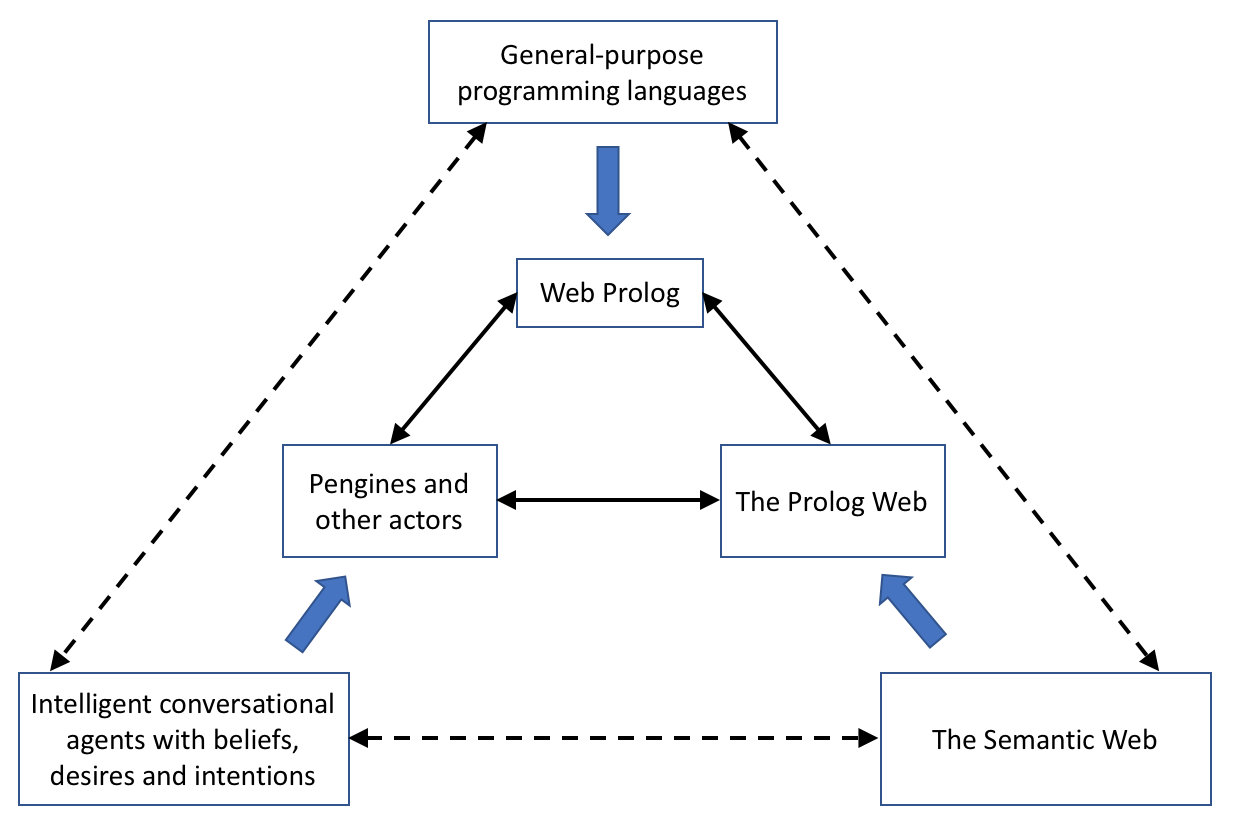
\includegraphics[width=7.5cm]{big-picture.png}
    \caption{The big picture. The different kinds of arrows can be interpreted in the following way: Thick and blue stands for \textit{simplification}; solid black for \textit{precisely defined dependencies}; dashed lines for \textit{vague dependencies}.}
    \label{fig:whole}
\end{figure}


\subsection{A Hierarchy of Useful Abstractions}\label{sec:hierarchy-of-abstraction}

\noindent In Web Prolog, just like in Erlang, the actor is regarded as the fundamental unit of computation and as the single abstraction that solves the two problems of concurrency and distribution and provides a form of network transparency. In Web Prolog, just like in Erlang, other network-transparent programming abstractions can be built on top of the actor. In Web Prolog, the most prominent and universally useful such abstraction is the pengine, followed closely by the abstraction for making non-deterministic remote procedure calls. These are both abstractions that would not fit easily into Erlang, but which are natural in Web Prolog. Abstractions such as these can be compared to Erlang \textit{behaviours}. They are not always easy to build, but once they are built they can easily be instantiated and tailored to specific tasks. 

We note that these three abstractions -- the actor, the pengine and the remote procedure call -- form a hierarchy where predicates on the higher levels inherit some of their options from predicates on the lower levels. \texttt{rpc/3} inherits options from \texttt{pengine\_spawn/2} and \texttt{pengine\_ask/3}, and \texttt{pengine\_spawn/2} inherits options from \texttt{spawn/3} in turn. 



%The node, populated by pengines and other actors, can perhaps be seen as yet another abstraction. When the stateless HTTP API is used to communicate with a node, the identities of any pengines involved are hidden.
%
%Finally, as we shall see, the Prolog Web can be seen as an abstraction as well.


\subsection{Web Prolog and the Programmable Prolog Web}\label{sec:for-erlangers-2}

\noindent A node has a dual identity. It can be seen not only as a Web Prolog runtime system but also as a node in the network forming what we will refer to as \textit{the Prolog Web}. The traditional Web is distributed, decentralised and open, and these are traits we want the Prolog Web to share. Whereas distribution is nicely conceptualised in the actor model, and nicely handled by an actor programming language such as Erlang or Web Prolog, decentralisation and openness require features we choose to rely on the Web as such to contribute.

Here, the humble URI is a key concept, as it allows us to link a Web Prolog program to another Web Prolog program, a running actor to another running actor, or a Prolog query to its answers, in much the same way as HTML documents are linked to other HTML documents.

Another key feature of the Prolog Web is that communication among nodes relies only on HTTP and the WebSocket protocol. This allows it to pass through firewalls, and provides security-related features such as methods for authentication, HTTPS and CORS (Cross-Origin Request Sharing).\footnote{\url{https://en.wikipedia.org/wiki/Cross-origin_resource_sharing}}

Distributed programming in Erlang typically involves a number of nodes connected into a cluster. Erlang nodes usually rely on TCP/IP for transport and are, for reasons of security, assumed to be operating in a closed, trusted environment where we directly control the machines involved. In other words, when Erlang runs on a cluster, it is a cluster that is \textit{closed}. In comparison, the Prolog Web might be seen as a cluster as well, but one that is as \textit{open} as the Web itself. %, and just as open as the Web itself.

%In the context of Web Prolog we can compare an Erlang cluster to what we refer to as \textit{the Prolog Web}. We think of the Prolog Web as an extension of the traditional Web, but it might be seen as a cluster as well, but one that is \textit{open}. 


%\subsection{Web Prolog and the programmable Prolog Web 2}\label{sec:for-erlangers-2}
%
%Distributed programming in Erlang typically involves a number of nodes connected into a cluster. Erlang nodes usually rely on TCP/IP for transport and are, for reasons of security, assumed to be operating in a closed, trusted environment where we directly control the machines involved. In other words, when Erlang runs on a cluster, it is a cluster that is \textit{closed}.
%
%In the context of Web Prolog we can compare an Erlang cluster to what we refer to as \textit{the Prolog Web}. We think of the Prolog Web as an extension of the traditional Web, but it might be seen as a cluster as well, but one that is \textit{open}. 
%
%The traditional Web is distributed, decentralised and open and these are traits we want the Prolog Web to inherit. Whereas distribution is nicely conceptualised in the actor model, and nicely handled by an actor programming language such as Erlang or Web Prolog, decentralisation and openness require features we choose to rely on the Web as such to contribute. 
%
%Here, the humble URI is a key concept, as it allows us to link a Web Prolog program to another Web Prolog program, a running actor to another running actor, or a Prolog query to its answers, in much the same way as HTML documents are linked to other HTML documents.
%
%The Prolog Web relies only on web APIs based on HTTP and the WebSocket protocol. This allows communication to pass through firewalls, and implements various security-related features such as methods for authentication, Secure websockets (i.e. websockets over HTTPS) and CORS (Cross-Origin Request Sharing).

%\footnote{\url{https://en.wikipedia.org/wiki/Cross-origin_resource_sharing}

%\vspace{-2mm}

\subsection{Would the Prolog Web Scale?}

\noindent By adopting a computational model capable of scaling out not only to multiple cores on one machine but also to multiple nodes running on multiple machines, by introducing an option allowing clients to limit the number of network roundtrips it takes to run a query to completion, by embracing the WebSocket transport protocol with its low overhead per message, by offering also a stateless HTTP API, and by leaving ample room for old as well as new forms of caching on both clients, nodes and intermediaries, we have made our best to ensure our high hopes for the scalability of the Prolog Web are not unfounded.

For the Prolog Web to be able to scale \textit{really} well, nodes must also be able to spawn very many actors, creating and destroying actors must be fast, and the communication among them efficient. Since actors created by the Erlang virtual machine are famous for having exactly those properties, this is certainly yet another reason for us to look closely at Erlang.
%, a language very well positioned to take advantage of the hardware multi-core revolution. 

An implementation of a Web Prolog node in Erlang might be interesting since it would most probably have a performance profile different from our implementation in SWI-Prolog. Interestingly, there is already Erlog -- a fairly complete Prolog implementation in Erlang written by Robert Virding -- which might serve as a point of departure.\footnote{\url{https://github.com/rvirding/erlog}} Erlog is an interpreter so the basic Prolog machinery (e.g. unification and backtracking) is likely to be slower in Erlog compared to (say) SWI-Prolog, whereas the super-fast lightweight processes of Erlang have other advantages, probably allowing it to scale better to very many simultaneous clients on a network. For the networking part, we note that Erlang is particularly famous for extremely efficient implementations of web-related technologies such as web servers (e.g. Yaws and Cowboy) and this could also be a distinctive advantage for an Erlang implementation of Web Prolog. 

The holy grail for a Web Prolog runtime system is a compiler targeting a virtual machine with BEAM-like properties, capable of producing code which when run will create processes as small and efficient as Erlang processes, yet with the useful capabilities that Prolog offers. We do not dare to guess whether building such a virtual machine is feasible.


\section{Rebranding Prolog}\label{sec:for-erlangers}

\begin{quote}
\textit{Rebranding} is a marketing strategy in which a new name, term, symbol, design, or combination thereof is created for an established brand with the intention of developing a new, differentiated identity in the minds of consumers, investors, competitors, and other stakeholders. 
\textit{Wikipedia}
\end{quote}

\vspace{2mm}

\noindent While the paradigms of imperative, functional and object-oriented programming have a vigorous following, the paradigm of logic programming with its flagship Prolog has fallen behind. People both inside and outside the community have at various occasions voiced their fears about the future of Prolog, noting that there are too many incompatible systems around, resulting in a fragmented community and an ISO standard that few systems conform to.

We suggest rebranding as a strategy for reviving Prolog, and offer Web Prolog in the hope that it may serve as a \textit{lingua franca} allowing different Prolog systems to communicate, and possibly aid the ``defragmentation'' of the community.

The strategy of rebranding as such is not a new idea. %In fact, we would suggest that Elixir might be regarded as a rebranded Erlang. Since Elixir appears to be more popular than Erlang, rebranding seems to have worked. However, since we do not propose to change the syntax of Prolog, only its purpose, our approach to rebranding is different.

%JavaScript must be regarded as \textit{the} web programming language of our times, but developers are starting to ask for other languages as well.\footnote{At least one leading engineer at Google thinks we need more web programming languages. See \url{https://www.pcworld.com/article/2362500/google-engineer-we-need-more-web-programming-languages.html}} With a language such as Elm, functional programming has been moving in this direction, but when it comes to logic programming languages, not much is happening.\footnote{But here is a promising attempt:  \url{https://rlaanemets.com/post/show/scripting-webpages-with-prolog-webassembly-and-virtual-dom}} Thus, when the Erlang community evaluates Web Prolog, it should not think about it as an alternative to Erlang, but rather as an alternative to JavaScript.


\section{Summary and Future Work}\label{sec:summary}

\noindent In accordance with our rebranding strategy, we choose to present our summary in the form of two ``elevator pitches''.

\vspace{0.3cm}

\begin{quote}
Imagine a dialect of Prolog with actors and mailboxes and send and receive -- all the means necessary for powerful concurrent and distributed programming.  Alternatively, think of it as a dialect of Erlang with logic variables, backtracking search and a built-in database of facts and rules -- the means for logic programming, knowledge representation and reasoning. Also, think of it as a web logic programming language. This is what Web Prolog is all about.
\flushright\textit{Web Prolog -- the elevator pitch}
\end{quote}

\vspace{0.2cm}

\begin{quote}
Imagine the Web wrapped in Prolog, running on top of a distributed architecture comprising a network of nodes supporting HTTP and WebSocket APIs, as well as web formats such as JSON. Think of it as a high-level Web, capable of serving answers to queries -- answers that follow from what the Web ``knows''. Moreover, imagine it being programmable, allowing Web Prolog source code to flow in either direction, from the client to the node or from the node to the client. This is what the Prolog Web is all about.
\vspace{2mm}
\flushright\textit{The Prolog Web -- the elevator pitch}
\end{quote}

\vspace{2mm}

\noindent Our work on the design and implementation of Web Prolog has so far resulted in a somewhat sketchy language specification and a proof-of-concept demonstrator featuring a fairly comprehensive interactive tutorial. As for future work, our next goal is to make sure the demonstrator is robust and secure enough to allow people to play with the language online without having to download anything.

In parallel to investing more work into building something that can be used in production, we are considering making an early attempt to create a standard for Web Prolog, based on a suitable subset of ISO Prolog, but developed under the auspices of the W3C this time rather than ISO, or under a liaison between these organisations. As a first move in this direction, we might create a W3C Community Group,\footnote{\url{https://www.w3.org/community}} as this appears to be an easy way to find out if enough interest can be generated among people of appropriate expertise.

A realistic but ambitious deadline for a standardisation effort would be to aim for 2022, the year when Prolog celebrates its 50th birthday. We find it difficult, in fact, to think of a better way to celebrate this occasion than to release version 1.0 of such a standard along with software implementing it.

%We believe that Prolog programmers might quickly realise that with Web Prolog they would be able to do things not easily done in traditional Prolog, and that Erlang programmers would find that Web Prolog offers interesting and useful capabilities that are not present in Erlang. 
 

We believe that Erlang technology might have something to contribute to Web Prolog, and, of course, that Prolog technology has something to contribute to Erlang (and by that we mean more than it has already contributed by once upon a time having inspired Erlang). 
Nowadays, there is not much contact between the Prolog community and the Erlang community. In the best of worlds, the language of Web Prolog might serve to open a new line of communication between the two communities.

As we now have not only logic, but also the Web in common, we have high hopes that some members in the Semantic Web community would like to join us in the celebration of the 50th birthday of Prolog.

\bibliography{pengines}

\end{document}

